\documentclass[twoside]{book}

% Packages required by doxygen
\usepackage{calc}
\usepackage{doxygen}
\usepackage{graphicx}
\usepackage[utf8]{inputenc}
\usepackage{makeidx}
\usepackage{multicol}
\usepackage{multirow}
\usepackage{textcomp}
\usepackage[table]{xcolor}

% Font selection
\usepackage[T1]{fontenc}
\usepackage{mathptmx}
\usepackage[scaled=.90]{helvet}
\usepackage{courier}
\usepackage{amssymb}
\usepackage{sectsty}
\renewcommand{\familydefault}{\sfdefault}
\allsectionsfont{%
  \fontseries{bc}\selectfont%
  \color{darkgray}%
}
\renewcommand{\DoxyLabelFont}{%
  \fontseries{bc}\selectfont%
  \color{darkgray}%
}

% Page & text layout
\usepackage{geometry}
\geometry{%
  a4paper,%
  top=2.5cm,%
  bottom=2.5cm,%
  left=2.5cm,%
  right=2.5cm%
}
\tolerance=750
\hfuzz=15pt
\hbadness=750
\setlength{\emergencystretch}{15pt}
\setlength{\parindent}{0cm}
\setlength{\parskip}{0.2cm}
\makeatletter
\renewcommand{\paragraph}{%
  \@startsection{paragraph}{4}{0ex}{-1.0ex}{1.0ex}{%
    \normalfont\normalsize\bfseries\SS@parafont%
  }%
}
\renewcommand{\subparagraph}{%
  \@startsection{subparagraph}{5}{0ex}{-1.0ex}{1.0ex}{%
    \normalfont\normalsize\bfseries\SS@subparafont%
  }%
}
\makeatother

% Headers & footers
\usepackage{fancyhdr}
\pagestyle{fancyplain}
\fancyhead[LE]{\fancyplain{}{\bfseries\thepage}}
\fancyhead[CE]{\fancyplain{}{}}
\fancyhead[RE]{\fancyplain{}{\bfseries\leftmark}}
\fancyhead[LO]{\fancyplain{}{\bfseries\rightmark}}
\fancyhead[CO]{\fancyplain{}{}}
\fancyhead[RO]{\fancyplain{}{\bfseries\thepage}}
\fancyfoot[LE]{\fancyplain{}{}}
\fancyfoot[CE]{\fancyplain{}{}}
\fancyfoot[RE]{\fancyplain{}{\bfseries\scriptsize Generated on Wed Aug 13 2014 11\-:55\-:37 for D\-N\-A Compression by K\-L-\/\-Substitutable Grammar Inference by Doxygen }}
\fancyfoot[LO]{\fancyplain{}{\bfseries\scriptsize Generated on Wed Aug 13 2014 11\-:55\-:37 for D\-N\-A Compression by K\-L-\/\-Substitutable Grammar Inference by Doxygen }}
\fancyfoot[CO]{\fancyplain{}{}}
\fancyfoot[RO]{\fancyplain{}{}}
\renewcommand{\footrulewidth}{0.4pt}
\renewcommand{\chaptermark}[1]{%
  \markboth{#1}{}%
}
\renewcommand{\sectionmark}[1]{%
  \markright{\thesection\ #1}%
}

% Indices & bibliography
\usepackage{natbib}
\usepackage[titles]{tocloft}
\setcounter{tocdepth}{3}
\setcounter{secnumdepth}{5}
\makeindex

% Hyperlinks (required, but should be loaded last)
\usepackage{ifpdf}
\ifpdf
  \usepackage[pdftex,pagebackref=true]{hyperref}
\else
  \usepackage[ps2pdf,pagebackref=true]{hyperref}
\fi
\hypersetup{%
  colorlinks=true,%
  linkcolor=blue,%
  citecolor=blue,%
  unicode%
}

% Custom commands
\newcommand{\clearemptydoublepage}{%
  \newpage{\pagestyle{empty}\cleardoublepage}%
}


%===== C O N T E N T S =====

\begin{document}

% Titlepage & ToC
\hypersetup{pageanchor=false}
\pagenumbering{roman}
\begin{titlepage}
\vspace*{7cm}
\begin{center}%
{\Large D\-N\-A Compression by K\-L-\/\-Substitutable Grammar Inference }\\
\vspace*{1cm}
{\large Generated by Doxygen 1.8.6}\\
\vspace*{0.5cm}
{\small Wed Aug 13 2014 11:55:37}\\
\end{center}
\end{titlepage}
\clearemptydoublepage
\tableofcontents
\clearemptydoublepage
\pagenumbering{arabic}
\hypersetup{pageanchor=true}

%--- Begin generated contents ---
\chapter{Hierarchical Index}
\section{Class Hierarchy}
This inheritance list is sorted roughly, but not completely, alphabetically\-:\begin{DoxyCompactList}
\item \contentsline{section}{Alphabet}{\pageref{classAlphabet}}{}
\item \contentsline{section}{Dencoder}{\pageref{classDencoder}}{}
\item enable\-\_\-shared\-\_\-from\-\_\-this\begin{DoxyCompactList}
\item \contentsline{section}{Sequence}{\pageref{classSequence}}{}
\end{DoxyCompactList}
\item \contentsline{section}{Grammar}{\pageref{classGrammar}}{}
\item \contentsline{section}{Non\-Terminal}{\pageref{classNonTerminal}}{}
\item \contentsline{section}{Production}{\pageref{classProduction}}{}
\item \contentsline{section}{Sub\-Sequence}{\pageref{classSubSequence}}{}
\begin{DoxyCompactList}
\item \contentsline{section}{Word}{\pageref{classWord}}{}
\end{DoxyCompactList}
\item \contentsline{section}{Suffix\-Array}{\pageref{classSuffixArray}}{}
\item \contentsline{section}{Symbol}{\pageref{classSymbol}}{}
\item \contentsline{section}{U\-Yi\-V}{\pageref{classUYiV}}{}
\item \contentsline{section}{Word\-List}{\pageref{classWordList}}{}
\end{DoxyCompactList}

\chapter{Class Index}
\section{Class List}
Here are the classes, structs, unions and interfaces with brief descriptions\-:\begin{DoxyCompactList}
\item\contentsline{section}{\hyperlink{classAlphabet}{Alphabet} }{\pageref{classAlphabet}}{}
\item\contentsline{section}{\hyperlink{classDencoder}{Dencoder} }{\pageref{classDencoder}}{}
\item\contentsline{section}{\hyperlink{classGrammar}{Grammar} }{\pageref{classGrammar}}{}
\item\contentsline{section}{\hyperlink{classNonTerminal}{Non\-Terminal} }{\pageref{classNonTerminal}}{}
\item\contentsline{section}{\hyperlink{classProduction}{Production} }{\pageref{classProduction}}{}
\item\contentsline{section}{\hyperlink{classSequence}{Sequence} }{\pageref{classSequence}}{}
\item\contentsline{section}{\hyperlink{classSubSequence}{Sub\-Sequence} }{\pageref{classSubSequence}}{}
\item\contentsline{section}{\hyperlink{classSuffixArray}{Suffix\-Array} }{\pageref{classSuffixArray}}{}
\item\contentsline{section}{\hyperlink{classSymbol}{Symbol} }{\pageref{classSymbol}}{}
\item\contentsline{section}{\hyperlink{classUYiV}{U\-Yi\-V} }{\pageref{classUYiV}}{}
\item\contentsline{section}{\hyperlink{classWord}{Word} }{\pageref{classWord}}{}
\item\contentsline{section}{\hyperlink{classWordList}{Word\-List} }{\pageref{classWordList}}{}
\end{DoxyCompactList}

\chapter{Class Documentation}
\hypertarget{classAlphabet}{\section{Alphabet Class Reference}
\label{classAlphabet}\index{Alphabet@{Alphabet}}
}
\subsection*{Public Member Functions}
\begin{DoxyCompactItemize}
\item 
\hyperlink{classAlphabet_aac9f2f615174ca6c8f89331239cb765e}{Alphabet} ()
\item 
\hyperlink{classAlphabet_a8a1da1bd7fdf2fd06a9768f9597a0b44}{$\sim$\-Alphabet} ()
\item 
void \hyperlink{classAlphabet_aedbea218764ce0b3a7a6c6c78c8bb512}{insert} (key k, value i)
\item 
int \hyperlink{classAlphabet_a549d8ebebef18a820f44c78d714fd57a}{get\-Size} () const 
\item 
bm\-\_\-type $\ast$ \hyperlink{classAlphabet_afd7f8853344abf9ffac03f5cd9926ab9}{get\-Alph\-Bi\-Map} () const 
\item 
value \hyperlink{classAlphabet_aaf6ac568ec863073cb5a053553b7a683}{get\-Value} (key k) const 
\item 
key \hyperlink{classAlphabet_ae9b301e2b793e74fad230f5ab66134da}{get\-Key} (value v) const 
\end{DoxyCompactItemize}
\subsection*{Friends}
\begin{DoxyCompactItemize}
\item 
ostream \& \hyperlink{classAlphabet_a4c763414b43f53cffd0537ba93827db8}{operator$<$$<$} (ostream \&cout, const \hyperlink{classAlphabet}{Alphabet} \&alph)
\end{DoxyCompactItemize}


\subsection{Constructor \& Destructor Documentation}
\hypertarget{classAlphabet_aac9f2f615174ca6c8f89331239cb765e}{\index{Alphabet@{Alphabet}!Alphabet@{Alphabet}}
\index{Alphabet@{Alphabet}!Alphabet@{Alphabet}}
\subsubsection[{Alphabet}]{\setlength{\rightskip}{0pt plus 5cm}Alphabet\-::\-Alphabet (
\begin{DoxyParamCaption}
{}
\end{DoxyParamCaption}
)}}\label{classAlphabet_aac9f2f615174ca6c8f89331239cb765e}
Create new bimap alphabet with (A,0),(C,1),(G,2), (T,3) key-\/values \hypertarget{classAlphabet_a8a1da1bd7fdf2fd06a9768f9597a0b44}{\index{Alphabet@{Alphabet}!$\sim$\-Alphabet@{$\sim$\-Alphabet}}
\index{$\sim$\-Alphabet@{$\sim$\-Alphabet}!Alphabet@{Alphabet}}
\subsubsection[{$\sim$\-Alphabet}]{\setlength{\rightskip}{0pt plus 5cm}Alphabet\-::$\sim$\-Alphabet (
\begin{DoxyParamCaption}
{}
\end{DoxyParamCaption}
)}}\label{classAlphabet_a8a1da1bd7fdf2fd06a9768f9597a0b44}
Delete alphabet\-\_\- 

\subsection{Member Function Documentation}
\hypertarget{classAlphabet_afd7f8853344abf9ffac03f5cd9926ab9}{\index{Alphabet@{Alphabet}!get\-Alph\-Bi\-Map@{get\-Alph\-Bi\-Map}}
\index{get\-Alph\-Bi\-Map@{get\-Alph\-Bi\-Map}!Alphabet@{Alphabet}}
\subsubsection[{get\-Alph\-Bi\-Map}]{\setlength{\rightskip}{0pt plus 5cm}bm\-\_\-type $\ast$ Alphabet\-::get\-Alph\-Bi\-Map (
\begin{DoxyParamCaption}
{}
\end{DoxyParamCaption}
) const}}\label{classAlphabet_afd7f8853344abf9ffac03f5cd9926ab9}
get the bimap data struct where the alphabet is buid in \begin{DoxyReturn}{Returns}
bimap alphabet\-\_\- 
\end{DoxyReturn}
\hypertarget{classAlphabet_ae9b301e2b793e74fad230f5ab66134da}{\index{Alphabet@{Alphabet}!get\-Key@{get\-Key}}
\index{get\-Key@{get\-Key}!Alphabet@{Alphabet}}
\subsubsection[{get\-Key}]{\setlength{\rightskip}{0pt plus 5cm}key Alphabet\-::get\-Key (
\begin{DoxyParamCaption}
\item[{value}]{v}
\end{DoxyParamCaption}
) const}}\label{classAlphabet_ae9b301e2b793e74fad230f5ab66134da}
get key from a given value 
\begin{DoxyParams}{Parameters}
{\em v} & value \\
\hline
\end{DoxyParams}
\begin{DoxyReturn}{Returns}
key 
\end{DoxyReturn}
\hypertarget{classAlphabet_a549d8ebebef18a820f44c78d714fd57a}{\index{Alphabet@{Alphabet}!get\-Size@{get\-Size}}
\index{get\-Size@{get\-Size}!Alphabet@{Alphabet}}
\subsubsection[{get\-Size}]{\setlength{\rightskip}{0pt plus 5cm}int Alphabet\-::get\-Size (
\begin{DoxyParamCaption}
{}
\end{DoxyParamCaption}
) const}}\label{classAlphabet_a549d8ebebef18a820f44c78d714fd57a}
Get \hyperlink{classAlphabet}{Alphabet} size \begin{DoxyReturn}{Returns}
int size\-\_\- 
\end{DoxyReturn}
\hypertarget{classAlphabet_aaf6ac568ec863073cb5a053553b7a683}{\index{Alphabet@{Alphabet}!get\-Value@{get\-Value}}
\index{get\-Value@{get\-Value}!Alphabet@{Alphabet}}
\subsubsection[{get\-Value}]{\setlength{\rightskip}{0pt plus 5cm}value Alphabet\-::get\-Value (
\begin{DoxyParamCaption}
\item[{key}]{k}
\end{DoxyParamCaption}
) const}}\label{classAlphabet_aaf6ac568ec863073cb5a053553b7a683}
get value from a given key 
\begin{DoxyParams}{Parameters}
{\em k} & key \\
\hline
\end{DoxyParams}
\begin{DoxyReturn}{Returns}
value 
\end{DoxyReturn}
\hypertarget{classAlphabet_aedbea218764ce0b3a7a6c6c78c8bb512}{\index{Alphabet@{Alphabet}!insert@{insert}}
\index{insert@{insert}!Alphabet@{Alphabet}}
\subsubsection[{insert}]{\setlength{\rightskip}{0pt plus 5cm}void Alphabet\-::insert (
\begin{DoxyParamCaption}
\item[{key}]{k, }
\item[{value}]{i}
\end{DoxyParamCaption}
)}}\label{classAlphabet_aedbea218764ce0b3a7a6c6c78c8bb512}
Insert new $<$k,value$>$ to the alphabet 
\begin{DoxyParams}{Parameters}
{\em k} & key \\
\hline
{\em i} & value \\
\hline
\end{DoxyParams}
\begin{DoxyReturn}{Returns}
value added or if already exist old value. 
\end{DoxyReturn}


\subsection{Friends And Related Function Documentation}
\hypertarget{classAlphabet_a4c763414b43f53cffd0537ba93827db8}{\index{Alphabet@{Alphabet}!operator$<$$<$@{operator$<$$<$}}
\index{operator$<$$<$@{operator$<$$<$}!Alphabet@{Alphabet}}
\subsubsection[{operator$<$$<$}]{\setlength{\rightskip}{0pt plus 5cm}ostream\& operator$<$$<$ (
\begin{DoxyParamCaption}
\item[{ostream \&}]{cout, }
\item[{const {\bf Alphabet} \&}]{alph}
\end{DoxyParamCaption}
)\hspace{0.3cm}{\ttfamily [friend]}}}\label{classAlphabet_a4c763414b43f53cffd0537ba93827db8}
Overload $<$$<$ operator to cout the \hyperlink{classAlphabet}{Alphabet} 

The documentation for this class was generated from the following files\-:\begin{DoxyCompactItemize}
\item 
Alphabet.\-h\item 
Alphabet.\-cpp\end{DoxyCompactItemize}

\hypertarget{classDencoder}{\section{Dencoder Class Reference}
\label{classDencoder}\index{Dencoder@{Dencoder}}
}
\subsection*{Public Member Functions}
\begin{DoxyCompactItemize}
\item 
\hyperlink{classDencoder_a5e50eb7f889e5d1880111bf4cd42985b}{Dencoder} ()
\item 
\hyperlink{classDencoder_a1d030025676e52628f911f9262bfc892}{$\sim$\-Dencoder} ()
\item 
void \hyperlink{classDencoder_af5dc170b4feaff7ed8743ce1f7c17582}{read\-Sequence} (const char $\ast$filename)
\item 
void \hyperlink{classDencoder_aebc51ef45ee13914e51627b04a07ea27}{update\-Sequence} (shared\-\_\-ptr$<$ \hyperlink{classSequence}{Sequence} $>$ new\-Seq)
\item 
shared\-\_\-ptr$<$ \hyperlink{classUYiV}{U\-Yi\-V} $>$ \hyperlink{classDencoder_a2da7de0ad2cea870406d318316090583}{create\-U\-Yi\-V\-From\-Maximal\-Repeats} (\hyperlink{classWordList}{Word\-List} $\ast$mrs)
\item 
shared\-\_\-ptr$<$ \hyperlink{classUYiV}{U\-Yi\-V} $>$ \hyperlink{classDencoder_ad73c4ee6f7eb88cd2ecee07514d26b92}{get\-Best\-U\-Yi\-V} (unordered\-\_\-set$<$ shared\-\_\-ptr$<$ \hyperlink{classWord}{Word} $>$ $>$ $\ast$ws) const 
\item 
double \hyperlink{classDencoder_acfb48805d38b387440332b4f98d02bec}{score} (shared\-\_\-ptr$<$ \hyperlink{classUYiV}{U\-Yi\-V} $>$ uyv) const 
\item 
double \hyperlink{classDencoder_acb61796bd459bb115b277cb249a05aac}{score} (shared\-\_\-ptr$<$ \hyperlink{classWord}{Word} $>$ w) const 
\item 
shared\-\_\-ptr$<$ \hyperlink{classUYiV}{U\-Yi\-V} $>$ \hyperlink{classDencoder_a6276f38e8d95fa8603a1fe80e6de504e}{best\-U\-V} (const list$<$ shared\-\_\-ptr$<$ \hyperlink{classUYiV}{U\-Yi\-V} $>$ $>$ $\ast$ls) const 
\item 
shared\-\_\-ptr$<$ \hyperlink{classWord}{Word} $>$ \hyperlink{classDencoder_ab538a82eb2e31be2ad8e10b6d02fa959}{best\-Word} (unordered\-\_\-set$<$ shared\-\_\-ptr$<$ \hyperlink{classWord}{Word} $>$ $>$ $\ast$us) const 
\item 
\hypertarget{classDencoder_ae6f7c6f84888d022589549979c4be3ea}{void {\bfseries recursion\-Replace} (shared\-\_\-ptr$<$ \hyperlink{classUYiV}{U\-Yi\-V} $>$ uyv)}\label{classDencoder_ae6f7c6f84888d022589549979c4be3ea}

\item 
\hypertarget{classDencoder_a4ee6f71a4466a853b19a78457c787c0c}{void {\bfseries update\-Word} (shared\-\_\-ptr$<$ \hyperlink{classSequence}{Sequence} $>$ seq, shared\-\_\-ptr$<$ \hyperlink{classWord}{Word} $>$ \&w)}\label{classDencoder_a4ee6f71a4466a853b19a78457c787c0c}

\item 
void \hyperlink{classDencoder_a1482876f6aa77c3d06aea0ded13b6a22}{get\-U\-V\-From\-Maximal\-Repeat} (shared\-\_\-ptr$<$ \hyperlink{classUYiV}{U\-Yi\-V} $>$ \&best, shared\-\_\-ptr$<$ \hyperlink{classWord}{Word} $>$ mr)
\item 
\hypertarget{classDencoder_aaa99f2ab3e47c3b7c40deb5c1eecc2f8}{int {\bfseries encoding\-Changes} (shared\-\_\-ptr$<$ \hyperlink{classUYiV}{U\-Yi\-V} $>$ uyv) const }\label{classDencoder_aaa99f2ab3e47c3b7c40deb5c1eecc2f8}

\item 
void \hyperlink{classDencoder_a6f277d3bf91144be89643626214c798e}{replace} (shared\-\_\-ptr$<$ \hyperlink{classUYiV}{U\-Yi\-V} $>$ uyv)
\item 
void \hyperlink{classDencoder_af79918dee8bfe223023356f586d6f21e}{replace\-Non\-Terminal} (shared\-\_\-ptr$<$ \hyperlink{classUYiV}{U\-Yi\-V} $>$ uyv, int non\-Terminal)
\item 
void \hyperlink{classDencoder_a6a796494a7caed55b71dd8c3e725ce3b}{replace\-Non\-Terminal\-Simple} (shared\-\_\-ptr$<$ \hyperlink{classUYiV}{U\-Yi\-V} $>$ uyv, int non\-Terminal)
\item 
void \hyperlink{classDencoder_a40dec7fcc058dbb18a7ee3f5729c5d95}{replace\-Non\-Terminal\-Word} (shared\-\_\-ptr$<$ \hyperlink{classWord}{Word} $>$ w, int non\-Terminal)
\item 
list$<$ shared\-\_\-ptr$<$ \hyperlink{classProduction}{Production} $>$ $>$ $\ast$ \hyperlink{classDencoder_a4a83e4396020fc47b969af504f3f4dee}{rebuild\-Grammar} (int $\ast$sec, vector$<$ int $>$ delimiter\-Pos, int total)
\item 
void \hyperlink{classDencoder_a58efab8245727d4cf284964907e047f8}{replace\-Word} (shared\-\_\-ptr$<$ \hyperlink{classWord}{Word} $>$ w)
\item 
void \hyperlink{classDencoder_aeda162ad58a07d6472878bf6dc31245e}{replace\-Yield} (shared\-\_\-ptr$<$ \hyperlink{classUYiV}{U\-Yi\-V} $>$ uyv)
\item 
void \hyperlink{classDencoder_a02caefcb12787c42d483e3fc3280441d}{replace\-Yield\-Simple} (shared\-\_\-ptr$<$ \hyperlink{classUYiV}{U\-Yi\-V} $>$ uyv)
\item 
void \hyperlink{classDencoder_ac54580ccea343b815ae0790d0d671a0c}{decode} ()
\item 
\hypertarget{classDencoder_aed77f2f64705826f2d91d2959da55761}{void {\bfseries dfs\-Enc} (int non\-Terminal, int start, int end, vector$<$ int $>$ \&enc)}\label{classDencoder_aed77f2f64705826f2d91d2959da55761}

\item 
shared\-\_\-ptr$<$ \hyperlink{classSequence}{Sequence} $>$ \hyperlink{classDencoder_a72a971a43c744b743485b6a2130d09a0}{get\-Seq\-Ori} () const 
\item 
shared\-\_\-ptr$<$ \hyperlink{classSequence}{Sequence} $>$ \hyperlink{classDencoder_aee23fb62f64684360a0bfc53a34e7774}{get\-Seq} () const 
\item 
\hyperlink{classSymbol}{Symbol} $\ast$ \hyperlink{classDencoder_abef2c3b60fa243c530aebf7633187d2d}{get\-Symbol} () const 
\item 
shared\-\_\-ptr$<$ \hyperlink{classGrammar}{Grammar} $>$ \hyperlink{classDencoder_a308586ca235e3cac1c63a2ae924c84ea}{get\-Grammar} () const 
\item 
queue$<$ int $>$ \& \hyperlink{classDencoder_aa1b80b0f842d7cca9bb4c02be6c7ba9d}{get\-Prod\-Election\-Order} (int non\-Terminal)
\item 
int \hyperlink{classDencoder_aafe24f8efee20570ef46e48e5627a9ba}{get\-Prod\-Election\-Size} () const 
\item 
void \hyperlink{classDencoder_a99625de506fedf9d41fdbdb42daf062a}{set\-Grammar} (shared\-\_\-ptr$<$ \hyperlink{classGrammar}{Grammar} $>$ g)
\end{DoxyCompactItemize}


\subsection{Constructor \& Destructor Documentation}
\hypertarget{classDencoder_a5e50eb7f889e5d1880111bf4cd42985b}{\index{Dencoder@{Dencoder}!Dencoder@{Dencoder}}
\index{Dencoder@{Dencoder}!Dencoder@{Dencoder}}
\subsubsection[{Dencoder}]{\setlength{\rightskip}{0pt plus 5cm}Dencoder\-::\-Dencoder (
\begin{DoxyParamCaption}
{}
\end{DoxyParamCaption}
)}}\label{classDencoder_a5e50eb7f889e5d1880111bf4cd42985b}
all ptr to N\-U\-L\-L \hypertarget{classDencoder_a1d030025676e52628f911f9262bfc892}{\index{Dencoder@{Dencoder}!$\sim$\-Dencoder@{$\sim$\-Dencoder}}
\index{$\sim$\-Dencoder@{$\sim$\-Dencoder}!Dencoder@{Dencoder}}
\subsubsection[{$\sim$\-Dencoder}]{\setlength{\rightskip}{0pt plus 5cm}Dencoder\-::$\sim$\-Dencoder (
\begin{DoxyParamCaption}
{}
\end{DoxyParamCaption}
)}}\label{classDencoder_a1d030025676e52628f911f9262bfc892}
Delete Sequences objects 

\subsection{Member Function Documentation}
\hypertarget{classDencoder_a6276f38e8d95fa8603a1fe80e6de504e}{\index{Dencoder@{Dencoder}!best\-U\-V@{best\-U\-V}}
\index{best\-U\-V@{best\-U\-V}!Dencoder@{Dencoder}}
\subsubsection[{best\-U\-V}]{\setlength{\rightskip}{0pt plus 5cm}shared\-\_\-ptr$<$ {\bf U\-Yi\-V} $>$ Dencoder\-::best\-U\-V (
\begin{DoxyParamCaption}
\item[{const list$<$ shared\-\_\-ptr$<$ {\bf U\-Yi\-V} $>$ $>$ $\ast$}]{ls}
\end{DoxyParamCaption}
) const}}\label{classDencoder_a6276f38e8d95fa8603a1fe80e6de504e}
Get the best u-\/v contexts based on a score function from the dencoder 
\begin{DoxyParams}{Parameters}
{\em ls} & list containing uyv \\
\hline
\end{DoxyParams}
\begin{DoxyReturn}{Returns}
best shared\-\_\-ptr$<$\-U\-Yi\-V$>$ 
\end{DoxyReturn}
\hypertarget{classDencoder_ab538a82eb2e31be2ad8e10b6d02fa959}{\index{Dencoder@{Dencoder}!best\-Word@{best\-Word}}
\index{best\-Word@{best\-Word}!Dencoder@{Dencoder}}
\subsubsection[{best\-Word}]{\setlength{\rightskip}{0pt plus 5cm}shared\-\_\-ptr$<$ {\bf Word} $>$ Dencoder\-::best\-Word (
\begin{DoxyParamCaption}
\item[{unordered\-\_\-set$<$ shared\-\_\-ptr$<$ {\bf Word} $>$ $>$ $\ast$}]{us}
\end{DoxyParamCaption}
) const}}\label{classDencoder_ab538a82eb2e31be2ad8e10b6d02fa959}
Get the best \hyperlink{classWord}{Word} based on a score function 
\begin{DoxyParams}{Parameters}
{\em us} & unordered set of words \\
\hline
\end{DoxyParams}
\begin{DoxyReturn}{Returns}
best word 
\end{DoxyReturn}
\hypertarget{classDencoder_a2da7de0ad2cea870406d318316090583}{\index{Dencoder@{Dencoder}!create\-U\-Yi\-V\-From\-Maximal\-Repeats@{create\-U\-Yi\-V\-From\-Maximal\-Repeats}}
\index{create\-U\-Yi\-V\-From\-Maximal\-Repeats@{create\-U\-Yi\-V\-From\-Maximal\-Repeats}!Dencoder@{Dencoder}}
\subsubsection[{create\-U\-Yi\-V\-From\-Maximal\-Repeats}]{\setlength{\rightskip}{0pt plus 5cm}shared\-\_\-ptr$<$ {\bf U\-Yi\-V} $>$ Dencoder\-::create\-U\-Yi\-V\-From\-Maximal\-Repeats (
\begin{DoxyParamCaption}
\item[{{\bf Word\-List} $\ast$}]{mrs}
\end{DoxyParamCaption}
)}}\label{classDencoder_a2da7de0ad2cea870406d318316090583}
Given a \hyperlink{classWordList}{Word\-List}, get the best Yield formed from one of those maximal repeats 
\begin{DoxyParams}{Parameters}
{\em mrs} & a word\-List \\
\hline
\end{DoxyParams}
\begin{DoxyReturn}{Returns}
best Yield founded based on score. 
\end{DoxyReturn}
\hypertarget{classDencoder_ac54580ccea343b815ae0790d0d671a0c}{\index{Dencoder@{Dencoder}!decode@{decode}}
\index{decode@{decode}!Dencoder@{Dencoder}}
\subsubsection[{decode}]{\setlength{\rightskip}{0pt plus 5cm}void Dencoder\-::decode (
\begin{DoxyParamCaption}
{}
\end{DoxyParamCaption}
)}}\label{classDencoder_ac54580ccea343b815ae0790d0d671a0c}
decode the grammar into the original sequence \begin{DoxyReturn}{Returns}
\hyperlink{classSequence}{Sequence} 
\end{DoxyReturn}
\hypertarget{classDencoder_ad73c4ee6f7eb88cd2ecee07514d26b92}{\index{Dencoder@{Dencoder}!get\-Best\-U\-Yi\-V@{get\-Best\-U\-Yi\-V}}
\index{get\-Best\-U\-Yi\-V@{get\-Best\-U\-Yi\-V}!Dencoder@{Dencoder}}
\subsubsection[{get\-Best\-U\-Yi\-V}]{\setlength{\rightskip}{0pt plus 5cm}shared\-\_\-ptr$<$ {\bf U\-Yi\-V} $>$ Dencoder\-::get\-Best\-U\-Yi\-V (
\begin{DoxyParamCaption}
\item[{unordered\-\_\-set$<$ shared\-\_\-ptr$<$ {\bf Word} $>$ $>$ $\ast$}]{ws}
\end{DoxyParamCaption}
) const}}\label{classDencoder_ad73c4ee6f7eb88cd2ecee07514d26b92}
Given a wordset create \hyperlink{classUYiV}{U\-Yi\-V} yields crossing them and return the best one 
\begin{DoxyParams}{Parameters}
{\em ws} & set of words \\
\hline
\end{DoxyParams}
\begin{DoxyReturn}{Returns}
best \hyperlink{classUYiV}{U\-Yi\-V} 
\end{DoxyReturn}
\hypertarget{classDencoder_a308586ca235e3cac1c63a2ae924c84ea}{\index{Dencoder@{Dencoder}!get\-Grammar@{get\-Grammar}}
\index{get\-Grammar@{get\-Grammar}!Dencoder@{Dencoder}}
\subsubsection[{get\-Grammar}]{\setlength{\rightskip}{0pt plus 5cm}shared\-\_\-ptr$<$ {\bf Grammar} $>$ Dencoder\-::get\-Grammar (
\begin{DoxyParamCaption}
{}
\end{DoxyParamCaption}
) const}}\label{classDencoder_a308586ca235e3cac1c63a2ae924c84ea}
get the \hyperlink{classGrammar}{Grammar} \begin{DoxyReturn}{Returns}
grammar\-\_\- 
\end{DoxyReturn}
\hypertarget{classDencoder_aa1b80b0f842d7cca9bb4c02be6c7ba9d}{\index{Dencoder@{Dencoder}!get\-Prod\-Election\-Order@{get\-Prod\-Election\-Order}}
\index{get\-Prod\-Election\-Order@{get\-Prod\-Election\-Order}!Dencoder@{Dencoder}}
\subsubsection[{get\-Prod\-Election\-Order}]{\setlength{\rightskip}{0pt plus 5cm}queue$<$ int $>$ \& Dencoder\-::get\-Prod\-Election\-Order (
\begin{DoxyParamCaption}
\item[{int}]{non\-Terminal}
\end{DoxyParamCaption}
)}}\label{classDencoder_aa1b80b0f842d7cca9bb4c02be6c7ba9d}
returns a reference to the non\-Terminal elections queue \hypertarget{classDencoder_aafe24f8efee20570ef46e48e5627a9ba}{\index{Dencoder@{Dencoder}!get\-Prod\-Election\-Size@{get\-Prod\-Election\-Size}}
\index{get\-Prod\-Election\-Size@{get\-Prod\-Election\-Size}!Dencoder@{Dencoder}}
\subsubsection[{get\-Prod\-Election\-Size}]{\setlength{\rightskip}{0pt plus 5cm}int Dencoder\-::get\-Prod\-Election\-Size (
\begin{DoxyParamCaption}
{}
\end{DoxyParamCaption}
) const}}\label{classDencoder_aafe24f8efee20570ef46e48e5627a9ba}
Get the total size of the elections queues \begin{DoxyReturn}{Returns}
total size 
\end{DoxyReturn}
\hypertarget{classDencoder_aee23fb62f64684360a0bfc53a34e7774}{\index{Dencoder@{Dencoder}!get\-Seq@{get\-Seq}}
\index{get\-Seq@{get\-Seq}!Dencoder@{Dencoder}}
\subsubsection[{get\-Seq}]{\setlength{\rightskip}{0pt plus 5cm}shared\-\_\-ptr$<$ {\bf Sequence} $>$ Dencoder\-::get\-Seq (
\begin{DoxyParamCaption}
{}
\end{DoxyParamCaption}
) const}}\label{classDencoder_aee23fb62f64684360a0bfc53a34e7774}
Get ptr to current \hyperlink{classSequence}{Sequence} if N\-U\-L\-L exit. \begin{DoxyReturn}{Returns}
ptr to current sequence 
\end{DoxyReturn}
\hypertarget{classDencoder_a72a971a43c744b743485b6a2130d09a0}{\index{Dencoder@{Dencoder}!get\-Seq\-Ori@{get\-Seq\-Ori}}
\index{get\-Seq\-Ori@{get\-Seq\-Ori}!Dencoder@{Dencoder}}
\subsubsection[{get\-Seq\-Ori}]{\setlength{\rightskip}{0pt plus 5cm}shared\-\_\-ptr$<$ {\bf Sequence} $>$ Dencoder\-::get\-Seq\-Ori (
\begin{DoxyParamCaption}
{}
\end{DoxyParamCaption}
) const}}\label{classDencoder_a72a971a43c744b743485b6a2130d09a0}
get ptr to the original \hyperlink{classSequence}{Sequence}. If N\-U\-L\-L exit. \begin{DoxyReturn}{Returns}
ptr to original sequence 
\end{DoxyReturn}
\hypertarget{classDencoder_abef2c3b60fa243c530aebf7633187d2d}{\index{Dencoder@{Dencoder}!get\-Symbol@{get\-Symbol}}
\index{get\-Symbol@{get\-Symbol}!Dencoder@{Dencoder}}
\subsubsection[{get\-Symbol}]{\setlength{\rightskip}{0pt plus 5cm}{\bf Symbol} $\ast$ Dencoder\-::get\-Symbol (
\begin{DoxyParamCaption}
{}
\end{DoxyParamCaption}
) const}}\label{classDencoder_abef2c3b60fa243c530aebf7633187d2d}
get the symbol \begin{DoxyReturn}{Returns}
symbol\-\_\- 
\end{DoxyReturn}
\hypertarget{classDencoder_a1482876f6aa77c3d06aea0ded13b6a22}{\index{Dencoder@{Dencoder}!get\-U\-V\-From\-Maximal\-Repeat@{get\-U\-V\-From\-Maximal\-Repeat}}
\index{get\-U\-V\-From\-Maximal\-Repeat@{get\-U\-V\-From\-Maximal\-Repeat}!Dencoder@{Dencoder}}
\subsubsection[{get\-U\-V\-From\-Maximal\-Repeat}]{\setlength{\rightskip}{0pt plus 5cm}void Dencoder\-::get\-U\-V\-From\-Maximal\-Repeat (
\begin{DoxyParamCaption}
\item[{shared\-\_\-ptr$<$ {\bf U\-Yi\-V} $>$ \&}]{best, }
\item[{shared\-\_\-ptr$<$ {\bf Word} $>$}]{mr}
\end{DoxyParamCaption}
)}}\label{classDencoder_a1482876f6aa77c3d06aea0ded13b6a22}
Given the current best Yield and a word, try to find a Yield with the suffix and prefix of this word that's better than the current one. 
\begin{DoxyParams}{Parameters}
{\em best} & current best yield \\
\hline
{\em mr} & word \\
\hline
\end{DoxyParams}
\hypertarget{classDencoder_af5dc170b4feaff7ed8743ce1f7c17582}{\index{Dencoder@{Dencoder}!read\-Sequence@{read\-Sequence}}
\index{read\-Sequence@{read\-Sequence}!Dencoder@{Dencoder}}
\subsubsection[{read\-Sequence}]{\setlength{\rightskip}{0pt plus 5cm}void Dencoder\-::read\-Sequence (
\begin{DoxyParamCaption}
\item[{const char $\ast$}]{filename}
\end{DoxyParamCaption}
)}}\label{classDencoder_af5dc170b4feaff7ed8743ce1f7c17582}
read the string in the file and convert it to an \hyperlink{classSequence}{Sequence} object. Points sequence\-Ori to it. 
\begin{DoxyParams}{Parameters}
{\em filename} & \\
\hline
\end{DoxyParams}
\hypertarget{classDencoder_a4a83e4396020fc47b969af504f3f4dee}{\index{Dencoder@{Dencoder}!rebuild\-Grammar@{rebuild\-Grammar}}
\index{rebuild\-Grammar@{rebuild\-Grammar}!Dencoder@{Dencoder}}
\subsubsection[{rebuild\-Grammar}]{\setlength{\rightskip}{0pt plus 5cm}list$<$ shared\-\_\-ptr$<$ {\bf Production} $>$ $>$ $\ast$ Dencoder\-::rebuild\-Grammar (
\begin{DoxyParamCaption}
\item[{int $\ast$}]{sec, }
\item[{vector$<$ int $>$}]{delimiter\-Pos, }
\item[{int}]{total}
\end{DoxyParamCaption}
)}}\label{classDencoder_a4a83e4396020fc47b969af504f3f4dee}
Rebuild the grammar based on a given int sequence. It iterates over the sec looking for the delimiters \$, when they are founded it means a new production must be created. 
\begin{DoxyParams}{Parameters}
{\em sec} & the int sequence \\
\hline
{\em delimiter\-Pos} & a vector telling where are the delimiters \\
\hline
{\em total} & the total size \\
\hline
\end{DoxyParams}
\begin{DoxyReturn}{Returns}
the grammar list of productions 
\end{DoxyReturn}
\hypertarget{classDencoder_a6f277d3bf91144be89643626214c798e}{\index{Dencoder@{Dencoder}!replace@{replace}}
\index{replace@{replace}!Dencoder@{Dencoder}}
\subsubsection[{replace}]{\setlength{\rightskip}{0pt plus 5cm}void Dencoder\-::replace (
\begin{DoxyParamCaption}
\item[{shared\-\_\-ptr$<$ {\bf U\-Yi\-V} $>$}]{uyv}
\end{DoxyParamCaption}
)}}\label{classDencoder_a6f277d3bf91144be89643626214c798e}
replace given yield in the sequence 
\begin{DoxyParams}{Parameters}
{\em uyv} & yield to be replaced \\
\hline
\end{DoxyParams}
\hypertarget{classDencoder_af79918dee8bfe223023356f586d6f21e}{\index{Dencoder@{Dencoder}!replace\-Non\-Terminal@{replace\-Non\-Terminal}}
\index{replace\-Non\-Terminal@{replace\-Non\-Terminal}!Dencoder@{Dencoder}}
\subsubsection[{replace\-Non\-Terminal}]{\setlength{\rightskip}{0pt plus 5cm}void Dencoder\-::replace\-Non\-Terminal (
\begin{DoxyParamCaption}
\item[{shared\-\_\-ptr$<$ {\bf U\-Yi\-V} $>$}]{uyv, }
\item[{int}]{non\-Terminal}
\end{DoxyParamCaption}
)}}\label{classDencoder_af79918dee8bfe223023356f586d6f21e}
replace the given shield with a \hyperlink{classNonTerminal}{Non\-Terminal} in the \hyperlink{classSequence}{Sequence} 
\begin{DoxyParams}{Parameters}
{\em uyv} & the yield to be replaced \\
\hline
{\em non\-Terminal} & \\
\hline
\end{DoxyParams}
\hypertarget{classDencoder_a6a796494a7caed55b71dd8c3e725ce3b}{\index{Dencoder@{Dencoder}!replace\-Non\-Terminal\-Simple@{replace\-Non\-Terminal\-Simple}}
\index{replace\-Non\-Terminal\-Simple@{replace\-Non\-Terminal\-Simple}!Dencoder@{Dencoder}}
\subsubsection[{replace\-Non\-Terminal\-Simple}]{\setlength{\rightskip}{0pt plus 5cm}void Dencoder\-::replace\-Non\-Terminal\-Simple (
\begin{DoxyParamCaption}
\item[{shared\-\_\-ptr$<$ {\bf U\-Yi\-V} $>$}]{uyv, }
\item[{int}]{non\-Terminal}
\end{DoxyParamCaption}
)}}\label{classDencoder_a6a796494a7caed55b71dd8c3e725ce3b}
replace given uyv yield by a non terminal. \hyperlink{classUYiV}{U\-Yi\-V} must have empty insides. It's similar to word replace. 
\begin{DoxyParams}{Parameters}
{\em uyv} & yield to replace \\
\hline
{\em non\-Terminal} & \\
\hline
\end{DoxyParams}
\hypertarget{classDencoder_a40dec7fcc058dbb18a7ee3f5729c5d95}{\index{Dencoder@{Dencoder}!replace\-Non\-Terminal\-Word@{replace\-Non\-Terminal\-Word}}
\index{replace\-Non\-Terminal\-Word@{replace\-Non\-Terminal\-Word}!Dencoder@{Dencoder}}
\subsubsection[{replace\-Non\-Terminal\-Word}]{\setlength{\rightskip}{0pt plus 5cm}void Dencoder\-::replace\-Non\-Terminal\-Word (
\begin{DoxyParamCaption}
\item[{shared\-\_\-ptr$<$ {\bf Word} $>$}]{w, }
\item[{int}]{non\-Terminal}
\end{DoxyParamCaption}
)}}\label{classDencoder_a40dec7fcc058dbb18a7ee3f5729c5d95}
replace a word by a non terminal in the sequence 
\begin{DoxyParams}{Parameters}
{\em w} & word to be replaced \\
\hline
{\em non\-Terminal} & \\
\hline
\end{DoxyParams}
\hypertarget{classDencoder_a58efab8245727d4cf284964907e047f8}{\index{Dencoder@{Dencoder}!replace\-Word@{replace\-Word}}
\index{replace\-Word@{replace\-Word}!Dencoder@{Dencoder}}
\subsubsection[{replace\-Word}]{\setlength{\rightskip}{0pt plus 5cm}void Dencoder\-::replace\-Word (
\begin{DoxyParamCaption}
\item[{shared\-\_\-ptr$<$ {\bf Word} $>$}]{w}
\end{DoxyParamCaption}
)}}\label{classDencoder_a58efab8245727d4cf284964907e047f8}
replace the given word by the next non terminal 
\begin{DoxyParams}{Parameters}
{\em w} & word to be replaced \\
\hline
\end{DoxyParams}
\hypertarget{classDencoder_aeda162ad58a07d6472878bf6dc31245e}{\index{Dencoder@{Dencoder}!replace\-Yield@{replace\-Yield}}
\index{replace\-Yield@{replace\-Yield}!Dencoder@{Dencoder}}
\subsubsection[{replace\-Yield}]{\setlength{\rightskip}{0pt plus 5cm}void Dencoder\-::replace\-Yield (
\begin{DoxyParamCaption}
\item[{shared\-\_\-ptr$<$ {\bf U\-Yi\-V} $>$}]{uyv}
\end{DoxyParamCaption}
)}}\label{classDencoder_aeda162ad58a07d6472878bf6dc31245e}
replace the given yield and generate the productions needed 
\begin{DoxyParams}{Parameters}
{\em uyv} & \\
\hline
\end{DoxyParams}
\hypertarget{classDencoder_a02caefcb12787c42d483e3fc3280441d}{\index{Dencoder@{Dencoder}!replace\-Yield\-Simple@{replace\-Yield\-Simple}}
\index{replace\-Yield\-Simple@{replace\-Yield\-Simple}!Dencoder@{Dencoder}}
\subsubsection[{replace\-Yield\-Simple}]{\setlength{\rightskip}{0pt plus 5cm}void Dencoder\-::replace\-Yield\-Simple (
\begin{DoxyParamCaption}
\item[{shared\-\_\-ptr$<$ {\bf U\-Yi\-V} $>$}]{uyv}
\end{DoxyParamCaption}
)}}\label{classDencoder_a02caefcb12787c42d483e3fc3280441d}
replace the given yield with Inside N\-U\-L\-L (simple repeat) and generate the productions needed 
\begin{DoxyParams}{Parameters}
{\em uyv} & \\
\hline
\end{DoxyParams}
\hypertarget{classDencoder_acfb48805d38b387440332b4f98d02bec}{\index{Dencoder@{Dencoder}!score@{score}}
\index{score@{score}!Dencoder@{Dencoder}}
\subsubsection[{score}]{\setlength{\rightskip}{0pt plus 5cm}double Dencoder\-::score (
\begin{DoxyParamCaption}
\item[{shared\-\_\-ptr$<$ {\bf U\-Yi\-V} $>$}]{uyv}
\end{DoxyParamCaption}
) const}}\label{classDencoder_acfb48805d38b387440332b4f98d02bec}
Calculate score of a given \hyperlink{classUYiV}{U\-Yi\-V}. The score is based on the formulas written in the inform. 
\begin{DoxyParams}{Parameters}
{\em uyv} & \\
\hline
\end{DoxyParams}
\begin{DoxyReturn}{Returns}
score 
\end{DoxyReturn}
\hypertarget{classDencoder_acb61796bd459bb115b277cb249a05aac}{\index{Dencoder@{Dencoder}!score@{score}}
\index{score@{score}!Dencoder@{Dencoder}}
\subsubsection[{score}]{\setlength{\rightskip}{0pt plus 5cm}double Dencoder\-::score (
\begin{DoxyParamCaption}
\item[{shared\-\_\-ptr$<$ {\bf Word} $>$}]{w}
\end{DoxyParamCaption}
) const}}\label{classDencoder_acb61796bd459bb115b277cb249a05aac}
Calculate score of a given \hyperlink{classWord}{Word}. The score is based on the formulas written in the inform. 
\begin{DoxyParams}{Parameters}
{\em word} & \\
\hline
\end{DoxyParams}
\begin{DoxyReturn}{Returns}
score 
\end{DoxyReturn}
\hypertarget{classDencoder_a99625de506fedf9d41fdbdb42daf062a}{\index{Dencoder@{Dencoder}!set\-Grammar@{set\-Grammar}}
\index{set\-Grammar@{set\-Grammar}!Dencoder@{Dencoder}}
\subsubsection[{set\-Grammar}]{\setlength{\rightskip}{0pt plus 5cm}void Dencoder\-::set\-Grammar (
\begin{DoxyParamCaption}
\item[{shared\-\_\-ptr$<$ {\bf Grammar} $>$}]{g}
\end{DoxyParamCaption}
)}}\label{classDencoder_a99625de506fedf9d41fdbdb42daf062a}
Set a new grammar 
\begin{DoxyParams}{Parameters}
{\em g} & new grammar \\
\hline
\end{DoxyParams}
\hypertarget{classDencoder_aebc51ef45ee13914e51627b04a07ea27}{\index{Dencoder@{Dencoder}!update\-Sequence@{update\-Sequence}}
\index{update\-Sequence@{update\-Sequence}!Dencoder@{Dencoder}}
\subsubsection[{update\-Sequence}]{\setlength{\rightskip}{0pt plus 5cm}void Dencoder\-::update\-Sequence (
\begin{DoxyParamCaption}
\item[{shared\-\_\-ptr$<$ {\bf Sequence} $>$}]{new\-Seq}
\end{DoxyParamCaption}
)}}\label{classDencoder_aebc51ef45ee13914e51627b04a07ea27}
update the \hyperlink{classSequence}{Sequence} with the given one. 
\begin{DoxyParams}{Parameters}
{\em new\-Seq} & \\
\hline
\end{DoxyParams}


The documentation for this class was generated from the following files\-:\begin{DoxyCompactItemize}
\item 
Dencoder.\-h\item 
Dencoder.\-cpp\end{DoxyCompactItemize}

\hypertarget{classGrammar}{\section{Grammar Class Reference}
\label{classGrammar}\index{Grammar@{Grammar}}
}
\subsection*{Public Member Functions}
\begin{DoxyCompactItemize}
\item 
\hyperlink{classGrammar_adc518572feacb51f9859556ba8c08502}{Grammar} (list$<$ shared\-\_\-ptr$<$ \hyperlink{classProduction}{Production} $>$ $>$ $\ast$prods)
\item 
\hyperlink{classGrammar_a60e8bade0190ee9830d9c600e4216b36}{$\sim$\-Grammar} ()
\item 
int $\ast$ \hyperlink{classGrammar_a359e8a4b597224f0c59594d9c8609cee}{convert\-To\-Int} () const 
\item 
void \hyperlink{classGrammar_a5fe32ff8e6c0842da64898a45ecc4798}{add\-Prod} (shared\-\_\-ptr$<$ \hyperlink{classProduction}{Production} $>$ p)
\item 
int \hyperlink{classGrammar_abb3247e1ddde3fbcbaa66c4ea6595f33}{get\-Size} () const 
\item 
list$<$ shared\-\_\-ptr$<$ \hyperlink{classProduction}{Production} $>$ $>$ $\ast$ \hyperlink{classGrammar_a694a03d8053bb9638acde4fcb82dbd53}{get\-Prods} () const 
\item 
void \hyperlink{classGrammar_a6755b33e54a291cbec28ad7d8af2961a}{unfold\-Non\-Terminal} (int non\-Terminal, queue$<$ int $>$ \&election\-Queue)
\item 
void \hyperlink{classGrammar_a23068f7d1fe5812b8c4bfe5c066e6f7b}{delete\-Prod} (shared\-\_\-ptr$<$ \hyperlink{classProduction}{Production} $>$ p)
\item 
shared\-\_\-ptr$<$ \hyperlink{classProduction}{Production} $>$ \hyperlink{classGrammar_af4e0db12fadf358531a511ca0832f5f1}{get\-Prod\-By\-L\-H\-S} (int lhs) const 
\end{DoxyCompactItemize}
\subsection*{Friends}
\begin{DoxyCompactItemize}
\item 
ostream \& \hyperlink{classGrammar_a54a3c8adc1ef211c3fc4b81e11884337}{operator$<$$<$} (ostream \&cout, const \hyperlink{classGrammar}{Grammar} \&g)
\end{DoxyCompactItemize}


\subsection{Constructor \& Destructor Documentation}
\hypertarget{classGrammar_adc518572feacb51f9859556ba8c08502}{\index{Grammar@{Grammar}!Grammar@{Grammar}}
\index{Grammar@{Grammar}!Grammar@{Grammar}}
\subsubsection[{Grammar}]{\setlength{\rightskip}{0pt plus 5cm}Grammar\-::\-Grammar (
\begin{DoxyParamCaption}
\item[{list$<$ shared\-\_\-ptr$<$ {\bf Production} $>$ $>$ $\ast$}]{prods}
\end{DoxyParamCaption}
)}}\label{classGrammar_adc518572feacb51f9859556ba8c08502}
Constructor 
\begin{DoxyParams}{Parameters}
{\em prods} & a list of \hyperlink{classProduction}{Production} \\
\hline
\end{DoxyParams}
\hypertarget{classGrammar_a60e8bade0190ee9830d9c600e4216b36}{\index{Grammar@{Grammar}!$\sim$\-Grammar@{$\sim$\-Grammar}}
\index{$\sim$\-Grammar@{$\sim$\-Grammar}!Grammar@{Grammar}}
\subsubsection[{$\sim$\-Grammar}]{\setlength{\rightskip}{0pt plus 5cm}Grammar\-::$\sim$\-Grammar (
\begin{DoxyParamCaption}
{}
\end{DoxyParamCaption}
)}}\label{classGrammar_a60e8bade0190ee9830d9c600e4216b36}
Destructor 

\subsection{Member Function Documentation}
\hypertarget{classGrammar_a5fe32ff8e6c0842da64898a45ecc4798}{\index{Grammar@{Grammar}!add\-Prod@{add\-Prod}}
\index{add\-Prod@{add\-Prod}!Grammar@{Grammar}}
\subsubsection[{add\-Prod}]{\setlength{\rightskip}{0pt plus 5cm}void Grammar\-::add\-Prod (
\begin{DoxyParamCaption}
\item[{shared\-\_\-ptr$<$ {\bf Production} $>$}]{p}
\end{DoxyParamCaption}
)}}\label{classGrammar_a5fe32ff8e6c0842da64898a45ecc4798}
Add a \hyperlink{classProduction}{Production} to the grammar 
\begin{DoxyParams}{Parameters}
{\em p} & production to be added \\
\hline
\end{DoxyParams}
\hypertarget{classGrammar_a359e8a4b597224f0c59594d9c8609cee}{\index{Grammar@{Grammar}!convert\-To\-Int@{convert\-To\-Int}}
\index{convert\-To\-Int@{convert\-To\-Int}!Grammar@{Grammar}}
\subsubsection[{convert\-To\-Int}]{\setlength{\rightskip}{0pt plus 5cm}int $\ast$ Grammar\-::convert\-To\-Int (
\begin{DoxyParamCaption}
{}
\end{DoxyParamCaption}
) const}}\label{classGrammar_a359e8a4b597224f0c59594d9c8609cee}
Convert the grammar to an int array \begin{DoxyReturn}{Returns}
int$\ast$ seq\-Grammar 
\end{DoxyReturn}
\hypertarget{classGrammar_a23068f7d1fe5812b8c4bfe5c066e6f7b}{\index{Grammar@{Grammar}!delete\-Prod@{delete\-Prod}}
\index{delete\-Prod@{delete\-Prod}!Grammar@{Grammar}}
\subsubsection[{delete\-Prod}]{\setlength{\rightskip}{0pt plus 5cm}void Grammar\-::delete\-Prod (
\begin{DoxyParamCaption}
\item[{shared\-\_\-ptr$<$ {\bf Production} $>$}]{p}
\end{DoxyParamCaption}
)}}\label{classGrammar_a23068f7d1fe5812b8c4bfe5c066e6f7b}
delete given production from grammar 
\begin{DoxyParams}{Parameters}
{\em p} & production to be deleted \\
\hline
\end{DoxyParams}
\hypertarget{classGrammar_af4e0db12fadf358531a511ca0832f5f1}{\index{Grammar@{Grammar}!get\-Prod\-By\-L\-H\-S@{get\-Prod\-By\-L\-H\-S}}
\index{get\-Prod\-By\-L\-H\-S@{get\-Prod\-By\-L\-H\-S}!Grammar@{Grammar}}
\subsubsection[{get\-Prod\-By\-L\-H\-S}]{\setlength{\rightskip}{0pt plus 5cm}shared\-\_\-ptr$<$ {\bf Production} $>$ Grammar\-::get\-Prod\-By\-L\-H\-S (
\begin{DoxyParamCaption}
\item[{int}]{lhs}
\end{DoxyParamCaption}
) const}}\label{classGrammar_af4e0db12fadf358531a511ca0832f5f1}
get a \hyperlink{classProduction}{Production} by its L\-H\-S 
\begin{DoxyParams}{Parameters}
{\em lhs} & a non\-Terminal \\
\hline
\end{DoxyParams}
\begin{DoxyReturn}{Returns}
production with such lhs 
\end{DoxyReturn}
\hypertarget{classGrammar_a694a03d8053bb9638acde4fcb82dbd53}{\index{Grammar@{Grammar}!get\-Prods@{get\-Prods}}
\index{get\-Prods@{get\-Prods}!Grammar@{Grammar}}
\subsubsection[{get\-Prods}]{\setlength{\rightskip}{0pt plus 5cm}list$<$ shared\-\_\-ptr$<$ {\bf Production} $>$ $>$ $\ast$ Grammar\-::get\-Prods (
\begin{DoxyParamCaption}
{}
\end{DoxyParamCaption}
) const}}\label{classGrammar_a694a03d8053bb9638acde4fcb82dbd53}
get \hyperlink{classGrammar}{Grammar} Productions \hypertarget{classGrammar_abb3247e1ddde3fbcbaa66c4ea6595f33}{\index{Grammar@{Grammar}!get\-Size@{get\-Size}}
\index{get\-Size@{get\-Size}!Grammar@{Grammar}}
\subsubsection[{get\-Size}]{\setlength{\rightskip}{0pt plus 5cm}int Grammar\-::get\-Size (
\begin{DoxyParamCaption}
{}
\end{DoxyParamCaption}
) const}}\label{classGrammar_abb3247e1ddde3fbcbaa66c4ea6595f33}
Get \hyperlink{classGrammar}{Grammar} size \begin{DoxyReturn}{Returns}
size\-\_\- 
\end{DoxyReturn}
\hypertarget{classGrammar_a6755b33e54a291cbec28ad7d8af2961a}{\index{Grammar@{Grammar}!unfold\-Non\-Terminal@{unfold\-Non\-Terminal}}
\index{unfold\-Non\-Terminal@{unfold\-Non\-Terminal}!Grammar@{Grammar}}
\subsubsection[{unfold\-Non\-Terminal}]{\setlength{\rightskip}{0pt plus 5cm}void Grammar\-::unfold\-Non\-Terminal (
\begin{DoxyParamCaption}
\item[{int}]{non\-Terminal, }
\item[{queue$<$ int $>$ \&}]{election\-Queue}
\end{DoxyParamCaption}
)}}\label{classGrammar_a6755b33e54a291cbec28ad7d8af2961a}
given a non\-Terminal, look for it in each \hyperlink{classProduction}{Production} and replace it by its right side 
\begin{DoxyParams}{Parameters}
{\em non\-Terminal} & non\-Terminal to be replaced \\
\hline
\end{DoxyParams}


\subsection{Friends And Related Function Documentation}
\hypertarget{classGrammar_a54a3c8adc1ef211c3fc4b81e11884337}{\index{Grammar@{Grammar}!operator$<$$<$@{operator$<$$<$}}
\index{operator$<$$<$@{operator$<$$<$}!Grammar@{Grammar}}
\subsubsection[{operator$<$$<$}]{\setlength{\rightskip}{0pt plus 5cm}ostream\& operator$<$$<$ (
\begin{DoxyParamCaption}
\item[{ostream \&}]{cout, }
\item[{const {\bf Grammar} \&}]{g}
\end{DoxyParamCaption}
)\hspace{0.3cm}{\ttfamily [friend]}}}\label{classGrammar_a54a3c8adc1ef211c3fc4b81e11884337}
cout overload for \hyperlink{classGrammar}{Grammar} 

The documentation for this class was generated from the following files\-:\begin{DoxyCompactItemize}
\item 
Grammar.\-h\item 
Grammar.\-cpp\end{DoxyCompactItemize}

\hypertarget{classNonTerminal}{\section{Non\-Terminal Class Reference}
\label{classNonTerminal}\index{Non\-Terminal@{Non\-Terminal}}
}
\subsection*{Public Member Functions}
\begin{DoxyCompactItemize}
\item 
\hypertarget{classNonTerminal_abb27b4da50abffd6f3eec58f85a88ae5}{{\bfseries Non\-Terminal} (int symbol)}\label{classNonTerminal_abb27b4da50abffd6f3eec58f85a88ae5}

\item 
\hypertarget{classNonTerminal_a86179d5eace904ea86f0cb2dc1a72916}{int {\bfseries get\-Symbol} () const }\label{classNonTerminal_a86179d5eace904ea86f0cb2dc1a72916}

\item 
\hypertarget{classNonTerminal_ab691c816bc4b6e91bd9f982c79c5901c}{void {\bfseries set\-Symbol} (int symbol)}\label{classNonTerminal_ab691c816bc4b6e91bd9f982c79c5901c}

\end{DoxyCompactItemize}


The documentation for this class was generated from the following files\-:\begin{DoxyCompactItemize}
\item 
Non\-Terminal.\-h\item 
Non\-Terminal.\-cpp\end{DoxyCompactItemize}

\hypertarget{classProduction}{\section{Production Class Reference}
\label{classProduction}\index{Production@{Production}}
}
\subsection*{Public Member Functions}
\begin{DoxyCompactItemize}
\item 
\hyperlink{classProduction_a92f0f1d1dbb5c68af2d6f8c89844d4ff}{Production} (int lhs, int $\ast$rhs, int size)
\item 
\hyperlink{classProduction_ab5b3060f9e0a2bc189844e426d693dab}{$\sim$\-Production} ()
\item 
void \hyperlink{classProduction_a4038d894f79a5a86c86a9c1d66040413}{unfold\-Non\-Terminal} (shared\-\_\-ptr$<$ \hyperlink{classProduction}{Production} $>$ n\-T, queue$<$ int $>$ \&election\-Queue)
\item 
vector$<$ int $>$ \hyperlink{classProduction_a5990c3ec3c934f4495bb6bb858584921}{get\-Option} (int opt) const 
\item 
\hypertarget{classProduction_aab0440acaa257a40d134a2158d5df777}{int {\bfseries get\-Election\-Start\-Pos} (int election) const }\label{classProduction_aab0440acaa257a40d134a2158d5df777}

\item 
\hypertarget{classProduction_a93f8128c95b20f4f59cbc817efb9d301}{int {\bfseries get\-Election\-End\-Pos} (int election) const }\label{classProduction_a93f8128c95b20f4f59cbc817efb9d301}

\item 
int \hyperlink{classProduction_a93ac262e02b0ccbb1947a00ee4781cb6}{get\-Size} () const 
\item 
int $\ast$ \hyperlink{classProduction_a31a72db90489bc566a819ef360cf23f0}{get\-R\-H\-S} () const 
\item 
int \hyperlink{classProduction_ab2dbdb2d626870e8b8f8a655f0d2f17a}{get\-L\-H\-S} () const 
\end{DoxyCompactItemize}
\subsection*{Friends}
\begin{DoxyCompactItemize}
\item 
ostream \& \hyperlink{classProduction_ad80a14935ba04d26e9067e3c388002d7}{operator$<$$<$} (ostream \&cout, const \hyperlink{classProduction}{Production} \&p)
\end{DoxyCompactItemize}


\subsection{Constructor \& Destructor Documentation}
\hypertarget{classProduction_a92f0f1d1dbb5c68af2d6f8c89844d4ff}{\index{Production@{Production}!Production@{Production}}
\index{Production@{Production}!Production@{Production}}
\subsubsection[{Production}]{\setlength{\rightskip}{0pt plus 5cm}Production\-::\-Production (
\begin{DoxyParamCaption}
\item[{int}]{lhs, }
\item[{int $\ast$}]{rhs, }
\item[{int}]{size}
\end{DoxyParamCaption}
)}}\label{classProduction_a92f0f1d1dbb5c68af2d6f8c89844d4ff}
Constructor 
\begin{DoxyParams}{Parameters}
{\em lhs} & left-\/hand side \\
\hline
{\em rhs} & right-\/hand side \\
\hline
{\em size} & $\vert$rhs$\vert$+1 \\
\hline
\end{DoxyParams}
\hypertarget{classProduction_ab5b3060f9e0a2bc189844e426d693dab}{\index{Production@{Production}!$\sim$\-Production@{$\sim$\-Production}}
\index{$\sim$\-Production@{$\sim$\-Production}!Production@{Production}}
\subsubsection[{$\sim$\-Production}]{\setlength{\rightskip}{0pt plus 5cm}Production\-::$\sim$\-Production (
\begin{DoxyParamCaption}
{}
\end{DoxyParamCaption}
)}}\label{classProduction_ab5b3060f9e0a2bc189844e426d693dab}
Destructor, delete rhs 

\subsection{Member Function Documentation}
\hypertarget{classProduction_ab2dbdb2d626870e8b8f8a655f0d2f17a}{\index{Production@{Production}!get\-L\-H\-S@{get\-L\-H\-S}}
\index{get\-L\-H\-S@{get\-L\-H\-S}!Production@{Production}}
\subsubsection[{get\-L\-H\-S}]{\setlength{\rightskip}{0pt plus 5cm}int Production\-::get\-L\-H\-S (
\begin{DoxyParamCaption}
{}
\end{DoxyParamCaption}
) const}}\label{classProduction_ab2dbdb2d626870e8b8f8a655f0d2f17a}
get \hyperlink{classProduction}{Production} lhs \begin{DoxyReturn}{Returns}
lhs\-\_\- 
\end{DoxyReturn}
\hypertarget{classProduction_a5990c3ec3c934f4495bb6bb858584921}{\index{Production@{Production}!get\-Option@{get\-Option}}
\index{get\-Option@{get\-Option}!Production@{Production}}
\subsubsection[{get\-Option}]{\setlength{\rightskip}{0pt plus 5cm}vector$<$ int $>$ Production\-::get\-Option (
\begin{DoxyParamCaption}
\item[{int}]{opt}
\end{DoxyParamCaption}
) const}}\label{classProduction_a5990c3ec3c934f4495bb6bb858584921}
if the production has many possible branches, return as a vector the one given by opt 
\begin{DoxyParams}{Parameters}
{\em opt} & option to return \\
\hline
\end{DoxyParams}
\begin{DoxyReturn}{Returns}
a vector containing the option 
\end{DoxyReturn}
\hypertarget{classProduction_a31a72db90489bc566a819ef360cf23f0}{\index{Production@{Production}!get\-R\-H\-S@{get\-R\-H\-S}}
\index{get\-R\-H\-S@{get\-R\-H\-S}!Production@{Production}}
\subsubsection[{get\-R\-H\-S}]{\setlength{\rightskip}{0pt plus 5cm}int $\ast$ Production\-::get\-R\-H\-S (
\begin{DoxyParamCaption}
{}
\end{DoxyParamCaption}
) const}}\label{classProduction_a31a72db90489bc566a819ef360cf23f0}
get \hyperlink{classProduction}{Production} rhs \begin{DoxyReturn}{Returns}
rhs\-\_\- 
\end{DoxyReturn}
\hypertarget{classProduction_a93ac262e02b0ccbb1947a00ee4781cb6}{\index{Production@{Production}!get\-Size@{get\-Size}}
\index{get\-Size@{get\-Size}!Production@{Production}}
\subsubsection[{get\-Size}]{\setlength{\rightskip}{0pt plus 5cm}int Production\-::get\-Size (
\begin{DoxyParamCaption}
{}
\end{DoxyParamCaption}
) const}}\label{classProduction_a93ac262e02b0ccbb1947a00ee4781cb6}
get \hyperlink{classProduction}{Production} size \begin{DoxyReturn}{Returns}
size\-\_\- ($\vert$rhs$\vert$+1) 
\end{DoxyReturn}
\hypertarget{classProduction_a4038d894f79a5a86c86a9c1d66040413}{\index{Production@{Production}!unfold\-Non\-Terminal@{unfold\-Non\-Terminal}}
\index{unfold\-Non\-Terminal@{unfold\-Non\-Terminal}!Production@{Production}}
\subsubsection[{unfold\-Non\-Terminal}]{\setlength{\rightskip}{0pt plus 5cm}void Production\-::unfold\-Non\-Terminal (
\begin{DoxyParamCaption}
\item[{shared\-\_\-ptr$<$ {\bf Production} $>$}]{n\-T, }
\item[{queue$<$ int $>$ \&}]{election\-Queue}
\end{DoxyParamCaption}
)}}\label{classProduction_a4038d894f79a5a86c86a9c1d66040413}
replace non\-Terminal by given rhs 
\begin{DoxyParams}{Parameters}
{\em non\-Terminal} & non terminal \\
\hline
{\em rhs} & rhs to replace non terminal \\
\hline
\end{DoxyParams}


\subsection{Friends And Related Function Documentation}
\hypertarget{classProduction_ad80a14935ba04d26e9067e3c388002d7}{\index{Production@{Production}!operator$<$$<$@{operator$<$$<$}}
\index{operator$<$$<$@{operator$<$$<$}!Production@{Production}}
\subsubsection[{operator$<$$<$}]{\setlength{\rightskip}{0pt plus 5cm}ostream\& operator$<$$<$ (
\begin{DoxyParamCaption}
\item[{ostream \&}]{cout, }
\item[{const {\bf Production} \&}]{p}
\end{DoxyParamCaption}
)\hspace{0.3cm}{\ttfamily [friend]}}}\label{classProduction_ad80a14935ba04d26e9067e3c388002d7}
Print \hyperlink{classProduction}{Production} 

The documentation for this class was generated from the following files\-:\begin{DoxyCompactItemize}
\item 
Production.\-h\item 
Production.\-cpp\end{DoxyCompactItemize}

\hypertarget{classSequence}{\section{Sequence Class Reference}
\label{classSequence}\index{Sequence@{Sequence}}
}
Inheritance diagram for Sequence\-:\begin{figure}[H]
\begin{center}
\leavevmode
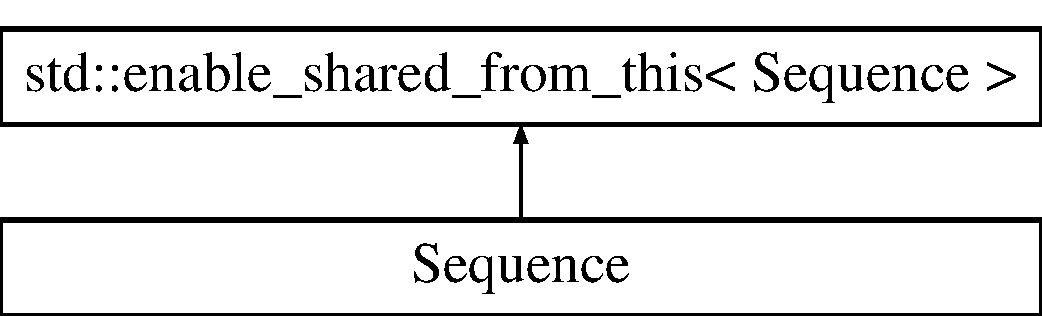
\includegraphics[height=2.000000cm]{classSequence}
\end{center}
\end{figure}
\subsection*{Public Member Functions}
\begin{DoxyCompactItemize}
\item 
list$<$ int $>$ $\ast$ \hyperlink{classSequence_a56c3dbd041ff758d1a2a0038c5ff4f43}{get\-Sub\-Seq\-Occ\-Pos} (const \hyperlink{classSubSequence}{Sub\-Sequence} $\ast$word, int s\-Array\-Start\-Index, int s\-Array\-End\-Index) const 
\item 
\hyperlink{classSequence_a532b7e8df6ff6b2f990c14ae97859ca2}{Sequence} ()
\item 
\hyperlink{classSequence_aee09a7d70c3ab523fed85da94ea1366f}{$\sim$\-Sequence} ()
\item 
int $\ast$ \hyperlink{classSequence_ac927b7e0d44e24a36014049a1d815971}{to\-Int} () const 
\item 
void \hyperlink{classSequence_a68148169be761cee0ab894e8a8926c43}{read\-From\-File} (const char $\ast$filename)
\item 
void \hyperlink{classSequence_a6902e3c6c47765dc91459f7df6234f33}{create\-From\-Int} (int $\ast$int\-Seq, int size)
\item 
std\-::shared\-\_\-ptr$<$ \hyperlink{classSequence}{Sequence} $>$ \hyperlink{classSequence_a116435038379ccab4e9f07d771e73235}{get\-Shared} ()
\item 
unordered\-\_\-set$<$ shared\-\_\-ptr\\*
$<$ \hyperlink{classWord}{Word} $>$ $>$ $\ast$ \hyperlink{classSequence_aee9c79f037c7638c637b1f851e6ec4a5}{maximal\-Repeats} ()
\item 
void \hyperlink{classSequence_aabde519f0689f9efa795f6a5c3d9416c}{create\-Words\-From\-Limits} (int seq\-Index, int length, unordered\-\_\-set$<$ shared\-\_\-ptr$<$ \hyperlink{classWord}{Word} $>$ $>$ $\ast$result)
\item 
void \hyperlink{classSequence_aedb4310b1b31e7b5866f40ce375dfe47}{get\-Separator\-Pos} (list$<$ int $>$ \&separator, int seq\-Index, int length)
\item 
list$<$ pair$<$ int, int $>$ $>$ $\ast$ \hyperlink{classSequence_af23046c26b6a8655bd98680f6f411f4a}{word\-Pos\-Pair\-List} (shared\-\_\-ptr$<$ \hyperlink{classWord}{Word} $>$ u, shared\-\_\-ptr$<$ \hyperlink{classWord}{Word} $>$ v) const 
\item 
\hyperlink{classWordList}{Word\-List} $\ast$ \hyperlink{classSequence_aa2e4d06d869c20f6b867c95d5e799c6b}{obtain\-Words\-Inside} (list$<$ std\-::pair$<$ int, int $>$ $>$ $\ast$pos\-Pairs, int u\-Size)
\item 
shared\-\_\-ptr$<$ \hyperlink{classWord}{Word} $>$ \hyperlink{classSequence_a4a48347d3684b23c75f92511256022e6}{create\-Sub\-Word} (shared\-\_\-ptr$<$ \hyperlink{classWord}{Word} $>$ w, int start, int end)
\item 
int \hyperlink{classSequence_af6bfa15998fba32a84eab8e0d969e7a1}{group\-Number} (int pos) const 
\item 
int \hyperlink{classSequence_a3ac0084617a2aee42b1514ae643cae55}{get\-Size} () const 
\item 
char $\ast$ \hyperlink{classSequence_abeffc3c8063c2053f558c91bd6c6ab03}{get\-Sequence} () const 
\item 
int $\ast$ \hyperlink{classSequence_a8494195fe7abb033a9aab325940117ad}{get\-Int\-Sequence} () const 
\item 
\hyperlink{classAlphabet}{Alphabet} $\ast$ \hyperlink{classSequence_a376651dcee5501a5f9f3a76020ffc463}{get\-Alphabet} () const 
\item 
\hyperlink{classSuffixArray}{Suffix\-Array} $\ast$ \hyperlink{classSequence_a4e964c20776c22b32d9e6ff88e6a4454}{get\-S\-Array} () const 
\item 
\hypertarget{classSequence_a72e78f8764e7f8774c45d137839eafc9}{int \& {\bfseries operator\mbox{[}$\,$\mbox{]}} (int idx)}\label{classSequence_a72e78f8764e7f8774c45d137839eafc9}

\item 
\hypertarget{classSequence_a307cc3236cd04a8669124763dd536c06}{const int \& {\bfseries operator\mbox{[}$\,$\mbox{]}} (int idx) const }\label{classSequence_a307cc3236cd04a8669124763dd536c06}

\end{DoxyCompactItemize}
\subsection*{Friends}
\begin{DoxyCompactItemize}
\item 
ostream \& \hyperlink{classSequence_a722cf4445d8ab47d57bb361498cee55d}{operator$<$$<$} (ostream \&cout, const \hyperlink{classSequence}{Sequence} \&seq)
\end{DoxyCompactItemize}


\subsection{Constructor \& Destructor Documentation}
\hypertarget{classSequence_a532b7e8df6ff6b2f990c14ae97859ca2}{\index{Sequence@{Sequence}!Sequence@{Sequence}}
\index{Sequence@{Sequence}!Sequence@{Sequence}}
\subsubsection[{Sequence}]{\setlength{\rightskip}{0pt plus 5cm}Sequence\-::\-Sequence (
\begin{DoxyParamCaption}
{}
\end{DoxyParamCaption}
)}}\label{classSequence_a532b7e8df6ff6b2f990c14ae97859ca2}
All ptrs to N\-U\-L\-L and size to 0 \hypertarget{classSequence_aee09a7d70c3ab523fed85da94ea1366f}{\index{Sequence@{Sequence}!$\sim$\-Sequence@{$\sim$\-Sequence}}
\index{$\sim$\-Sequence@{$\sim$\-Sequence}!Sequence@{Sequence}}
\subsubsection[{$\sim$\-Sequence}]{\setlength{\rightskip}{0pt plus 5cm}Sequence\-::$\sim$\-Sequence (
\begin{DoxyParamCaption}
{}
\end{DoxyParamCaption}
)}}\label{classSequence_aee09a7d70c3ab523fed85da94ea1366f}
Delete s\-Array\-\_\-, Sequences\-\_\- and alph\-\_\- 

\subsection{Member Function Documentation}
\hypertarget{classSequence_a6902e3c6c47765dc91459f7df6234f33}{\index{Sequence@{Sequence}!create\-From\-Int@{create\-From\-Int}}
\index{create\-From\-Int@{create\-From\-Int}!Sequence@{Sequence}}
\subsubsection[{create\-From\-Int}]{\setlength{\rightskip}{0pt plus 5cm}void Sequence\-::create\-From\-Int (
\begin{DoxyParamCaption}
\item[{int $\ast$}]{int\-Seq, }
\item[{int}]{size}
\end{DoxyParamCaption}
)}}\label{classSequence_a6902e3c6c47765dc91459f7df6234f33}
Read a file containing a string and complete the attributes of the \hyperlink{classSequence}{Sequence} object 
\begin{DoxyParams}{Parameters}
{\em filename} & with string create a \hyperlink{classSequence}{Sequence} object from an int array \\
\hline
{\em int\-Seq} & array \\
\hline
{\em size} & size of the array \\
\hline
\end{DoxyParams}
\hypertarget{classSequence_a4a48347d3684b23c75f92511256022e6}{\index{Sequence@{Sequence}!create\-Sub\-Word@{create\-Sub\-Word}}
\index{create\-Sub\-Word@{create\-Sub\-Word}!Sequence@{Sequence}}
\subsubsection[{create\-Sub\-Word}]{\setlength{\rightskip}{0pt plus 5cm}shared\-\_\-ptr$<$ {\bf Word} $>$ Sequence\-::create\-Sub\-Word (
\begin{DoxyParamCaption}
\item[{shared\-\_\-ptr$<$ {\bf Word} $>$}]{w, }
\item[{int}]{start, }
\item[{int}]{end}
\end{DoxyParamCaption}
)}}\label{classSequence_a4a48347d3684b23c75f92511256022e6}
Given a word create a subword of it given a start and an end index 
\begin{DoxyParams}{Parameters}
{\em w} & word \\
\hline
{\em start} & \\
\hline
{\em end} & \\
\hline
\end{DoxyParams}
\begin{DoxyReturn}{Returns}
subword 
\end{DoxyReturn}
\hypertarget{classSequence_aabde519f0689f9efa795f6a5c3d9416c}{\index{Sequence@{Sequence}!create\-Words\-From\-Limits@{create\-Words\-From\-Limits}}
\index{create\-Words\-From\-Limits@{create\-Words\-From\-Limits}!Sequence@{Sequence}}
\subsubsection[{create\-Words\-From\-Limits}]{\setlength{\rightskip}{0pt plus 5cm}void Sequence\-::create\-Words\-From\-Limits (
\begin{DoxyParamCaption}
\item[{int}]{seq\-Index, }
\item[{int}]{length, }
\item[{unordered\-\_\-set$<$ shared\-\_\-ptr$<$ {\bf Word} $>$ $>$ $\ast$}]{result}
\end{DoxyParamCaption}
)}}\label{classSequence_aabde519f0689f9efa795f6a5c3d9416c}
Create words based on delimiters in the sequence. Given and index and a length, check if it has a delimiter in the middle and creates words separated by those delimiters. 
\begin{DoxyParams}{Parameters}
{\em seq\-Index} & index in the sequence \\
\hline
{\em length} & length \\
\hline
{\em result} & set of words \\
\hline
\end{DoxyParams}
\hypertarget{classSequence_a376651dcee5501a5f9f3a76020ffc463}{\index{Sequence@{Sequence}!get\-Alphabet@{get\-Alphabet}}
\index{get\-Alphabet@{get\-Alphabet}!Sequence@{Sequence}}
\subsubsection[{get\-Alphabet}]{\setlength{\rightskip}{0pt plus 5cm}{\bf Alphabet} $\ast$ Sequence\-::get\-Alphabet (
\begin{DoxyParamCaption}
{}
\end{DoxyParamCaption}
) const}}\label{classSequence_a376651dcee5501a5f9f3a76020ffc463}
get the \hyperlink{classAlphabet}{Alphabet} \begin{DoxyReturn}{Returns}
alph\-\_\- 
\end{DoxyReturn}
\hypertarget{classSequence_a8494195fe7abb033a9aab325940117ad}{\index{Sequence@{Sequence}!get\-Int\-Sequence@{get\-Int\-Sequence}}
\index{get\-Int\-Sequence@{get\-Int\-Sequence}!Sequence@{Sequence}}
\subsubsection[{get\-Int\-Sequence}]{\setlength{\rightskip}{0pt plus 5cm}int $\ast$ Sequence\-::get\-Int\-Sequence (
\begin{DoxyParamCaption}
{}
\end{DoxyParamCaption}
) const}}\label{classSequence_a8494195fe7abb033a9aab325940117ad}
get \hyperlink{classSequence}{Sequence} in int \begin{DoxyReturn}{Returns}
int$\ast$ int\-Sequence\-\_\- 
\end{DoxyReturn}
\hypertarget{classSequence_a4e964c20776c22b32d9e6ff88e6a4454}{\index{Sequence@{Sequence}!get\-S\-Array@{get\-S\-Array}}
\index{get\-S\-Array@{get\-S\-Array}!Sequence@{Sequence}}
\subsubsection[{get\-S\-Array}]{\setlength{\rightskip}{0pt plus 5cm}{\bf Suffix\-Array} $\ast$ Sequence\-::get\-S\-Array (
\begin{DoxyParamCaption}
{}
\end{DoxyParamCaption}
) const}}\label{classSequence_a4e964c20776c22b32d9e6ff88e6a4454}
get the s\-Array \begin{DoxyReturn}{Returns}
\hyperlink{classSuffixArray}{Suffix\-Array} 
\end{DoxyReturn}
\hypertarget{classSequence_aedb4310b1b31e7b5866f40ce375dfe47}{\index{Sequence@{Sequence}!get\-Separator\-Pos@{get\-Separator\-Pos}}
\index{get\-Separator\-Pos@{get\-Separator\-Pos}!Sequence@{Sequence}}
\subsubsection[{get\-Separator\-Pos}]{\setlength{\rightskip}{0pt plus 5cm}void Sequence\-::get\-Separator\-Pos (
\begin{DoxyParamCaption}
\item[{list$<$ int $>$ \&}]{separator, }
\item[{int}]{seq\-Index, }
\item[{int}]{length}
\end{DoxyParamCaption}
)}}\label{classSequence_aedb4310b1b31e7b5866f40ce375dfe47}
Get the positions of the separatos starting from the index and finishin in index+length, it could be pipes or \$ 
\begin{DoxyParams}{Parameters}
{\em separator} & list of separatos \\
\hline
{\em seq\-Index} & index in the seq \\
\hline
{\em length} & length \\
\hline
\end{DoxyParams}
\hypertarget{classSequence_abeffc3c8063c2053f558c91bd6c6ab03}{\index{Sequence@{Sequence}!get\-Sequence@{get\-Sequence}}
\index{get\-Sequence@{get\-Sequence}!Sequence@{Sequence}}
\subsubsection[{get\-Sequence}]{\setlength{\rightskip}{0pt plus 5cm}char $\ast$ Sequence\-::get\-Sequence (
\begin{DoxyParamCaption}
{}
\end{DoxyParamCaption}
) const}}\label{classSequence_abeffc3c8063c2053f558c91bd6c6ab03}
get \hyperlink{classSequence}{Sequence} in char$\ast$ \begin{DoxyReturn}{Returns}
char$\ast$ sequence\-\_\- 
\end{DoxyReturn}
\hypertarget{classSequence_a116435038379ccab4e9f07d771e73235}{\index{Sequence@{Sequence}!get\-Shared@{get\-Shared}}
\index{get\-Shared@{get\-Shared}!Sequence@{Sequence}}
\subsubsection[{get\-Shared}]{\setlength{\rightskip}{0pt plus 5cm}std\-::shared\-\_\-ptr$<$ {\bf Sequence} $>$ Sequence\-::get\-Shared (
\begin{DoxyParamCaption}
{}
\end{DoxyParamCaption}
)}}\label{classSequence_a116435038379ccab4e9f07d771e73235}
get shared ptr from this \hypertarget{classSequence_a3ac0084617a2aee42b1514ae643cae55}{\index{Sequence@{Sequence}!get\-Size@{get\-Size}}
\index{get\-Size@{get\-Size}!Sequence@{Sequence}}
\subsubsection[{get\-Size}]{\setlength{\rightskip}{0pt plus 5cm}int Sequence\-::get\-Size (
\begin{DoxyParamCaption}
{}
\end{DoxyParamCaption}
) const}}\label{classSequence_a3ac0084617a2aee42b1514ae643cae55}
Get \hyperlink{classSequence}{Sequence} size \begin{DoxyReturn}{Returns}
int size 
\end{DoxyReturn}
\hypertarget{classSequence_a56c3dbd041ff758d1a2a0038c5ff4f43}{\index{Sequence@{Sequence}!get\-Sub\-Seq\-Occ\-Pos@{get\-Sub\-Seq\-Occ\-Pos}}
\index{get\-Sub\-Seq\-Occ\-Pos@{get\-Sub\-Seq\-Occ\-Pos}!Sequence@{Sequence}}
\subsubsection[{get\-Sub\-Seq\-Occ\-Pos}]{\setlength{\rightskip}{0pt plus 5cm}list$<$ int $>$ $\ast$ Sequence\-::get\-Sub\-Seq\-Occ\-Pos (
\begin{DoxyParamCaption}
\item[{const {\bf Sub\-Sequence} $\ast$}]{word, }
\item[{int}]{s\-Array\-Start\-Index, }
\item[{int}]{s\-Array\-End\-Index}
\end{DoxyParamCaption}
) const}}\label{classSequence_a56c3dbd041ff758d1a2a0038c5ff4f43}
get all occs in order of a given sub\-Seq 
\begin{DoxyParams}{Parameters}
{\em sub\-Seq} & a subsequence from the \hyperlink{classSequence}{Sequence}. \\
\hline
\end{DoxyParams}
\begin{DoxyReturn}{Returns}
list of occs positions. 
\end{DoxyReturn}
\hypertarget{classSequence_af6bfa15998fba32a84eab8e0d969e7a1}{\index{Sequence@{Sequence}!group\-Number@{group\-Number}}
\index{group\-Number@{group\-Number}!Sequence@{Sequence}}
\subsubsection[{group\-Number}]{\setlength{\rightskip}{0pt plus 5cm}int Sequence\-::group\-Number (
\begin{DoxyParamCaption}
\item[{int}]{pos}
\end{DoxyParamCaption}
) const}}\label{classSequence_af6bfa15998fba32a84eab8e0d969e7a1}
each group is separated by a delimiter (pipe or \$), return the group number of a given pos in the sequence 
\begin{DoxyParams}{Parameters}
{\em pos} & \\
\hline
\end{DoxyParams}
\begin{DoxyReturn}{Returns}
group number 
\end{DoxyReturn}
\hypertarget{classSequence_aee9c79f037c7638c637b1f851e6ec4a5}{\index{Sequence@{Sequence}!maximal\-Repeats@{maximal\-Repeats}}
\index{maximal\-Repeats@{maximal\-Repeats}!Sequence@{Sequence}}
\subsubsection[{maximal\-Repeats}]{\setlength{\rightskip}{0pt plus 5cm}unordered\-\_\-set$<$ shared\-\_\-ptr$<$ {\bf Word} $>$ $>$ $\ast$ Sequence\-::maximal\-Repeats (
\begin{DoxyParamCaption}
{}
\end{DoxyParamCaption}
)}}\label{classSequence_aee9c79f037c7638c637b1f851e6ec4a5}
Get all maximal repeats from the \hyperlink{classSequence}{Sequence} \begin{DoxyReturn}{Returns}
a ptr to \hyperlink{classWordList}{Word\-List} that are maximal repeats words 
\end{DoxyReturn}
\hypertarget{classSequence_aa2e4d06d869c20f6b867c95d5e799c6b}{\index{Sequence@{Sequence}!obtain\-Words\-Inside@{obtain\-Words\-Inside}}
\index{obtain\-Words\-Inside@{obtain\-Words\-Inside}!Sequence@{Sequence}}
\subsubsection[{obtain\-Words\-Inside}]{\setlength{\rightskip}{0pt plus 5cm}{\bf Word\-List} $\ast$ Sequence\-::obtain\-Words\-Inside (
\begin{DoxyParamCaption}
\item[{list$<$ std\-::pair$<$ int, int $>$ $>$ $\ast$}]{pos\-Pairs, }
\item[{int}]{u\-Size}
\end{DoxyParamCaption}
)}}\label{classSequence_aa2e4d06d869c20f6b867c95d5e799c6b}
obtain a \hyperlink{classWordList}{Word\-List} from all the Words within the pos\-Pairs list given 
\begin{DoxyParams}{Parameters}
{\em pos\-Pairs} & positions from contexts u and v \\
\hline
{\em u\-Size} & size of u context \\
\hline
{\em v\-Size} & size of v context \\
\hline
\end{DoxyParams}
\begin{DoxyReturn}{Returns}
\hyperlink{classWordList}{Word\-List} of all insides words 
\end{DoxyReturn}
\hypertarget{classSequence_a68148169be761cee0ab894e8a8926c43}{\index{Sequence@{Sequence}!read\-From\-File@{read\-From\-File}}
\index{read\-From\-File@{read\-From\-File}!Sequence@{Sequence}}
\subsubsection[{read\-From\-File}]{\setlength{\rightskip}{0pt plus 5cm}void Sequence\-::read\-From\-File (
\begin{DoxyParamCaption}
\item[{const char $\ast$}]{filename}
\end{DoxyParamCaption}
)}}\label{classSequence_a68148169be761cee0ab894e8a8926c43}
read a sequence from a given filename, takes token separate by spaces. 
\begin{DoxyParams}{Parameters}
{\em filename} & \\
\hline
\end{DoxyParams}
\hypertarget{classSequence_ac927b7e0d44e24a36014049a1d815971}{\index{Sequence@{Sequence}!to\-Int@{to\-Int}}
\index{to\-Int@{to\-Int}!Sequence@{Sequence}}
\subsubsection[{to\-Int}]{\setlength{\rightskip}{0pt plus 5cm}int $\ast$ Sequence\-::to\-Int (
\begin{DoxyParamCaption}
{}
\end{DoxyParamCaption}
) const}}\label{classSequence_ac927b7e0d44e24a36014049a1d815971}
Obtain an int sequence from the \hyperlink{classSequence}{Sequence} object. Uses this-\/$>$alph\-\_\- to translate the chars to int \begin{DoxyReturn}{Returns}
int\-Seq 
\end{DoxyReturn}
\hypertarget{classSequence_af23046c26b6a8655bd98680f6f411f4a}{\index{Sequence@{Sequence}!word\-Pos\-Pair\-List@{word\-Pos\-Pair\-List}}
\index{word\-Pos\-Pair\-List@{word\-Pos\-Pair\-List}!Sequence@{Sequence}}
\subsubsection[{word\-Pos\-Pair\-List}]{\setlength{\rightskip}{0pt plus 5cm}list$<$ pair$<$ int, int $>$ $>$ $\ast$ Sequence\-::word\-Pos\-Pair\-List (
\begin{DoxyParamCaption}
\item[{shared\-\_\-ptr$<$ {\bf Word} $>$}]{u, }
\item[{shared\-\_\-ptr$<$ {\bf Word} $>$}]{v}
\end{DoxyParamCaption}
) const}}\label{classSequence_af23046c26b6a8655bd98680f6f411f4a}
given two Words, return one list with no overlapped pairs of these words pos in the follow way\-: took the first element y from v\-Pos. Look for the max x in u\-Pos, with x+u\-Size$<$y. (x,y) is a pair in the res list. 
\begin{DoxyParams}{Parameters}
{\em u} & \\
\hline
{\em v} & \\
\hline
\end{DoxyParams}
\begin{DoxyReturn}{Returns}
list$<$pair\-Pos$>$ pairs representing a context, it can be N\-U\-L\-L 
\end{DoxyReturn}


\subsection{Friends And Related Function Documentation}
\hypertarget{classSequence_a722cf4445d8ab47d57bb361498cee55d}{\index{Sequence@{Sequence}!operator$<$$<$@{operator$<$$<$}}
\index{operator$<$$<$@{operator$<$$<$}!Sequence@{Sequence}}
\subsubsection[{operator$<$$<$}]{\setlength{\rightskip}{0pt plus 5cm}ostream\& operator$<$$<$ (
\begin{DoxyParamCaption}
\item[{ostream \&}]{cout, }
\item[{const {\bf Sequence} \&}]{seq}
\end{DoxyParamCaption}
)\hspace{0.3cm}{\ttfamily [friend]}}}\label{classSequence_a722cf4445d8ab47d57bb361498cee55d}
Overload $<$$<$ operator to cout the \hyperlink{classSequence}{Sequence} 

The documentation for this class was generated from the following files\-:\begin{DoxyCompactItemize}
\item 
Sequence.\-h\item 
Sequence.\-cpp\end{DoxyCompactItemize}

\hypertarget{classSubSequence}{\section{Sub\-Sequence Class Reference}
\label{classSubSequence}\index{Sub\-Sequence@{Sub\-Sequence}}
}
Inheritance diagram for Sub\-Sequence\-:\begin{figure}[H]
\begin{center}
\leavevmode
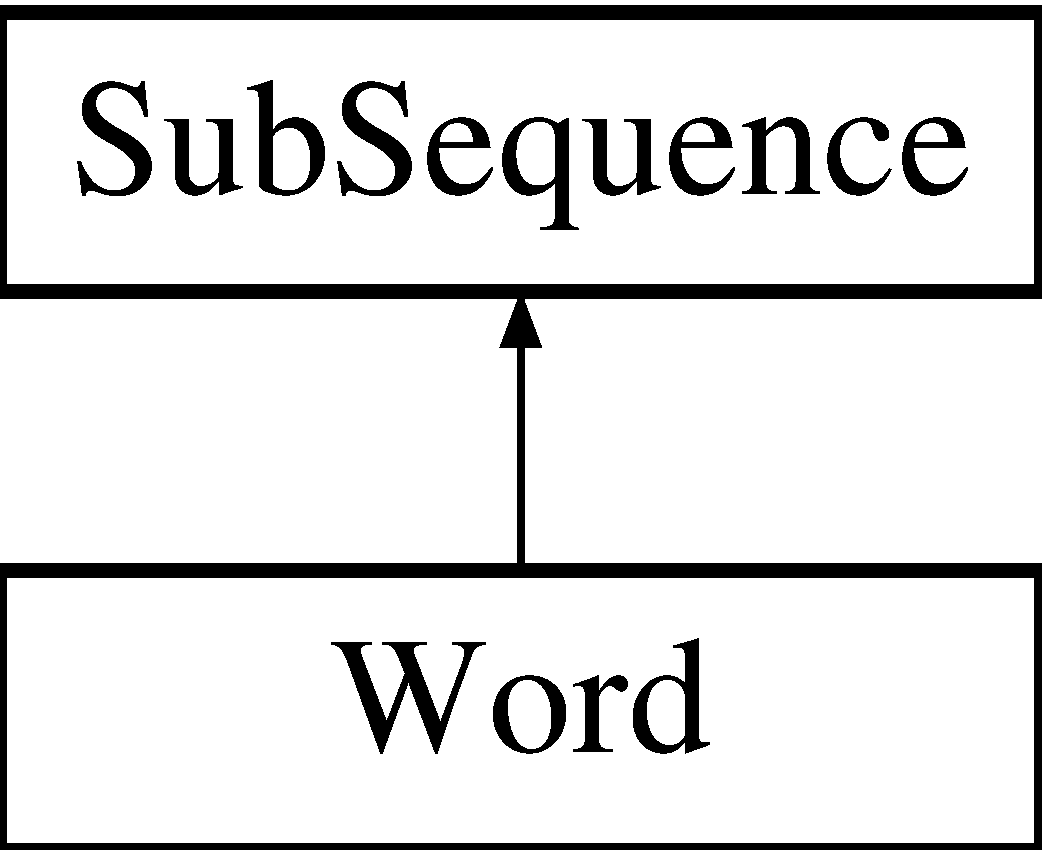
\includegraphics[height=2.000000cm]{classSubSequence}
\end{center}
\end{figure}
\subsection*{Public Member Functions}
\begin{DoxyCompactItemize}
\item 
\hyperlink{classSubSequence_a655d0a3b46af9b6bf646d37708221668}{Sub\-Sequence} (shared\-\_\-ptr$<$ \hyperlink{classSequence}{Sequence} $>$ mother\-Seq, const int start, const int end)
\item 
\hyperlink{classSubSequence_a8b9442f5f1d03952c5a0491f6dac0f63}{$\sim$\-Sub\-Sequence} ()
\item 
int $\ast$ \hyperlink{classSubSequence_aef9b8911ccfcc690a46734afad4fa2f1}{extract\-Range\-From\-Sequence} (const shared\-\_\-ptr$<$ \hyperlink{classSequence}{Sequence} $>$ mother\-Seq, const int start, const int end) const 
\item 
char $\ast$ \hyperlink{classSubSequence_ad53b4e7176f666ca97841850c7d25a38}{extract\-Range\-From\-Char\-Sequence} (const shared\-\_\-ptr$<$ \hyperlink{classSequence}{Sequence} $>$ mother\-Seq, const int start, const int end) const 
\item 
bool \hyperlink{classSubSequence_a2fab95b3b19abbcce7450b7c5c5ef169}{is\-Invalid} () const 
\item 
int \hyperlink{classSubSequence_a9d468d8c8e06ed55bbbfaead2fc16b4d}{get\-Size} () const 
\item 
int $\ast$ \hyperlink{classSubSequence_a3b17db4593e36945699c662510a6dded}{get\-Sub\-Sequence} () const 
\item 
bool \hyperlink{classSubSequence_a360b7b8f15252a929575c67ac43f6203}{operator==} (const \hyperlink{classSubSequence}{Sub\-Sequence} \&other) const 
\end{DoxyCompactItemize}
\subsection*{Friends}
\begin{DoxyCompactItemize}
\item 
ostream \& \hyperlink{classSubSequence_af7f3c998197b1785cee5d549df007173}{operator$<$$<$} (ostream \&cout, const \hyperlink{classSubSequence}{Sub\-Sequence} \&seq)
\end{DoxyCompactItemize}


\subsection{Constructor \& Destructor Documentation}
\hypertarget{classSubSequence_a655d0a3b46af9b6bf646d37708221668}{\index{Sub\-Sequence@{Sub\-Sequence}!Sub\-Sequence@{Sub\-Sequence}}
\index{Sub\-Sequence@{Sub\-Sequence}!SubSequence@{Sub\-Sequence}}
\subsubsection[{Sub\-Sequence}]{\setlength{\rightskip}{0pt plus 5cm}Sub\-Sequence\-::\-Sub\-Sequence (
\begin{DoxyParamCaption}
\item[{shared\-\_\-ptr$<$ {\bf Sequence} $>$}]{mother\-Seq, }
\item[{const int}]{start, }
\item[{const int}]{end}
\end{DoxyParamCaption}
)}}\label{classSubSequence_a655d0a3b46af9b6bf646d37708221668}
Given a sequence, do the logic to find a a subsequence of it and construct a \hyperlink{classSubSequence}{Sub\-Sequence} object. It's \mbox{[}start, end) 
\begin{DoxyParams}{Parameters}
{\em mother\-Seq} & \\
\hline
{\em start,a} & start index of the subsequence \\
\hline
{\em end,an} & end index, the closest to start \\
\hline
\end{DoxyParams}
\hypertarget{classSubSequence_a8b9442f5f1d03952c5a0491f6dac0f63}{\index{Sub\-Sequence@{Sub\-Sequence}!$\sim$\-Sub\-Sequence@{$\sim$\-Sub\-Sequence}}
\index{$\sim$\-Sub\-Sequence@{$\sim$\-Sub\-Sequence}!SubSequence@{Sub\-Sequence}}
\subsubsection[{$\sim$\-Sub\-Sequence}]{\setlength{\rightskip}{0pt plus 5cm}Sub\-Sequence\-::$\sim$\-Sub\-Sequence (
\begin{DoxyParamCaption}
{}
\end{DoxyParamCaption}
)}}\label{classSubSequence_a8b9442f5f1d03952c5a0491f6dac0f63}
delete sub\-Sequence. mother\-Seq is deleted in \hyperlink{classSequence}{Sequence} destructor 

\subsection{Member Function Documentation}
\hypertarget{classSubSequence_ad53b4e7176f666ca97841850c7d25a38}{\index{Sub\-Sequence@{Sub\-Sequence}!extract\-Range\-From\-Char\-Sequence@{extract\-Range\-From\-Char\-Sequence}}
\index{extract\-Range\-From\-Char\-Sequence@{extract\-Range\-From\-Char\-Sequence}!SubSequence@{Sub\-Sequence}}
\subsubsection[{extract\-Range\-From\-Char\-Sequence}]{\setlength{\rightskip}{0pt plus 5cm}char $\ast$ Sub\-Sequence\-::extract\-Range\-From\-Char\-Sequence (
\begin{DoxyParamCaption}
\item[{const shared\-\_\-ptr$<$ {\bf Sequence} $>$}]{mother\-Seq, }
\item[{const int}]{start, }
\item[{const int}]{end}
\end{DoxyParamCaption}
) const}}\label{classSubSequence_ad53b4e7176f666ca97841850c7d25a38}
given a range (start-\/end), extract the characters within this range from the sequence 
\begin{DoxyParams}{Parameters}
{\em mother\-Seq} & sequence \\
\hline
{\em start} & \\
\hline
{\em end} & \\
\hline
\end{DoxyParams}
\begin{DoxyReturn}{Returns}
characters in range 
\end{DoxyReturn}
\hypertarget{classSubSequence_aef9b8911ccfcc690a46734afad4fa2f1}{\index{Sub\-Sequence@{Sub\-Sequence}!extract\-Range\-From\-Sequence@{extract\-Range\-From\-Sequence}}
\index{extract\-Range\-From\-Sequence@{extract\-Range\-From\-Sequence}!SubSequence@{Sub\-Sequence}}
\subsubsection[{extract\-Range\-From\-Sequence}]{\setlength{\rightskip}{0pt plus 5cm}int $\ast$ Sub\-Sequence\-::extract\-Range\-From\-Sequence (
\begin{DoxyParamCaption}
\item[{const shared\-\_\-ptr$<$ {\bf Sequence} $>$}]{mother\-Seq, }
\item[{const int}]{start, }
\item[{const int}]{end}
\end{DoxyParamCaption}
) const}}\label{classSubSequence_aef9b8911ccfcc690a46734afad4fa2f1}
extract an int subsequence delimited by a range from the sequence 
\begin{DoxyParams}{Parameters}
{\em mother\-Seq} & sequence from we extract \\
\hline
{\em start} & start index \\
\hline
{\em end} & end index \\
\hline
\end{DoxyParams}
\begin{DoxyReturn}{Returns}
return in subsequence 
\end{DoxyReturn}
\hypertarget{classSubSequence_a9d468d8c8e06ed55bbbfaead2fc16b4d}{\index{Sub\-Sequence@{Sub\-Sequence}!get\-Size@{get\-Size}}
\index{get\-Size@{get\-Size}!SubSequence@{Sub\-Sequence}}
\subsubsection[{get\-Size}]{\setlength{\rightskip}{0pt plus 5cm}int Sub\-Sequence\-::get\-Size (
\begin{DoxyParamCaption}
{}
\end{DoxyParamCaption}
) const}}\label{classSubSequence_a9d468d8c8e06ed55bbbfaead2fc16b4d}
get the size of the subsequence \begin{DoxyReturn}{Returns}
int size\-\_\- 
\end{DoxyReturn}
\hypertarget{classSubSequence_a3b17db4593e36945699c662510a6dded}{\index{Sub\-Sequence@{Sub\-Sequence}!get\-Sub\-Sequence@{get\-Sub\-Sequence}}
\index{get\-Sub\-Sequence@{get\-Sub\-Sequence}!SubSequence@{Sub\-Sequence}}
\subsubsection[{get\-Sub\-Sequence}]{\setlength{\rightskip}{0pt plus 5cm}int $\ast$ Sub\-Sequence\-::get\-Sub\-Sequence (
\begin{DoxyParamCaption}
{}
\end{DoxyParamCaption}
) const}}\label{classSubSequence_a3b17db4593e36945699c662510a6dded}
get the int representation of the subsequence \begin{DoxyReturn}{Returns}
int$\ast$ sub\-Sequence\-\_\- 
\end{DoxyReturn}
\hypertarget{classSubSequence_a2fab95b3b19abbcce7450b7c5c5ef169}{\index{Sub\-Sequence@{Sub\-Sequence}!is\-Invalid@{is\-Invalid}}
\index{is\-Invalid@{is\-Invalid}!SubSequence@{Sub\-Sequence}}
\subsubsection[{is\-Invalid}]{\setlength{\rightskip}{0pt plus 5cm}bool Sub\-Sequence\-::is\-Invalid (
\begin{DoxyParamCaption}
{}
\end{DoxyParamCaption}
) const}}\label{classSubSequence_a2fab95b3b19abbcce7450b7c5c5ef169}
Say if a subsequence is invalid (if it has a pipe or a \$ is invalid) \begin{DoxyReturn}{Returns}
true if invalid 
\end{DoxyReturn}
\hypertarget{classSubSequence_a360b7b8f15252a929575c67ac43f6203}{\index{Sub\-Sequence@{Sub\-Sequence}!operator==@{operator==}}
\index{operator==@{operator==}!SubSequence@{Sub\-Sequence}}
\subsubsection[{operator==}]{\setlength{\rightskip}{0pt plus 5cm}bool Sub\-Sequence\-::operator== (
\begin{DoxyParamCaption}
\item[{const {\bf Sub\-Sequence} \&}]{other}
\end{DoxyParamCaption}
) const}}\label{classSubSequence_a360b7b8f15252a929575c67ac43f6203}
equality overloading. Be careful, just check if both has the same characters in the same order, but no if they are in the same position of mother\-Sequence. Complexity\-: O($\vert$left sub\-Sequence$\vert$) 

\subsection{Friends And Related Function Documentation}
\hypertarget{classSubSequence_af7f3c998197b1785cee5d549df007173}{\index{Sub\-Sequence@{Sub\-Sequence}!operator$<$$<$@{operator$<$$<$}}
\index{operator$<$$<$@{operator$<$$<$}!SubSequence@{Sub\-Sequence}}
\subsubsection[{operator$<$$<$}]{\setlength{\rightskip}{0pt plus 5cm}ostream\& operator$<$$<$ (
\begin{DoxyParamCaption}
\item[{ostream \&}]{cout, }
\item[{const {\bf Sub\-Sequence} \&}]{seq}
\end{DoxyParamCaption}
)\hspace{0.3cm}{\ttfamily [friend]}}}\label{classSubSequence_af7f3c998197b1785cee5d549df007173}
Overload $<$$<$ operator to cout the \hyperlink{classSubSequence}{Sub\-Sequence} 

The documentation for this class was generated from the following files\-:\begin{DoxyCompactItemize}
\item 
Sub\-Sequence.\-h\item 
Sub\-Sequence.\-cpp\end{DoxyCompactItemize}

\hypertarget{classSuffixArray}{\section{Suffix\-Array Class Reference}
\label{classSuffixArray}\index{Suffix\-Array@{Suffix\-Array}}
}
\subsection*{Public Member Functions}
\begin{DoxyCompactItemize}
\item 
\hyperlink{classSuffixArray_a83235ab312aea1c50ab3a616c85ae405}{Suffix\-Array} (int $\ast$seq, int size, bool larsson, int max\-Alph=-\/1)
\item 
\hyperlink{classSuffixArray_a6493c8516e4b76cce6fe0bfca47b13b0}{$\sim$\-Suffix\-Array} ()
\item 
\hypertarget{classSuffixArray_a1886977617bfc4c9cb7d6c643ebb0696}{pair$<$ int, int $>$ {\bfseries search} (int $\ast$s, int size)}\label{classSuffixArray_a1886977617bfc4c9cb7d6c643ebb0696}

\item 
int \hyperlink{classSuffixArray_a42c1557b2ad51886208dcf74b200e276}{get\-Size} () const 
\item 
int $\ast$ \hyperlink{classSuffixArray_a9f702b7c059a694cad1c776dd90b637a}{get\-S\-Array} () const 
\item 
int $\ast$ \hyperlink{classSuffixArray_a4ec9f2035ee2a6ed06ccbba58165c7e2}{get\-L\-C\-P} () const 
\item 
\hypertarget{classSuffixArray_a3a714f4d1d641c769b75957ef4f6c083}{int \& {\bfseries operator\mbox{[}$\,$\mbox{]}} (int idx)}\label{classSuffixArray_a3a714f4d1d641c769b75957ef4f6c083}

\item 
\hypertarget{classSuffixArray_a4b20c30605bb5244ff8efb02f53686d8}{const int \& {\bfseries operator\mbox{[}$\,$\mbox{]}} (int idx) const }\label{classSuffixArray_a4b20c30605bb5244ff8efb02f53686d8}

\end{DoxyCompactItemize}
\subsection*{Friends}
\begin{DoxyCompactItemize}
\item 
ostream \& \hyperlink{classSuffixArray_a79797b488f2191d1fef54a6eb01dce3f}{operator$<$$<$} (ostream \&cout, \hyperlink{classSuffixArray}{Suffix\-Array} \&s\-Array)
\end{DoxyCompactItemize}


\subsection{Constructor \& Destructor Documentation}
\hypertarget{classSuffixArray_a83235ab312aea1c50ab3a616c85ae405}{\index{Suffix\-Array@{Suffix\-Array}!Suffix\-Array@{Suffix\-Array}}
\index{Suffix\-Array@{Suffix\-Array}!SuffixArray@{Suffix\-Array}}
\subsubsection[{Suffix\-Array}]{\setlength{\rightskip}{0pt plus 5cm}Suffix\-Array\-::\-Suffix\-Array (
\begin{DoxyParamCaption}
\item[{int $\ast$}]{seq, }
\item[{int}]{size, }
\item[{bool}]{larsson, }
\item[{int}]{max\-Alph = {\ttfamily -\/1}}
\end{DoxyParamCaption}
)}}\label{classSuffixArray_a83235ab312aea1c50ab3a616c85ae405}
Construct s\-Array based on 
\begin{DoxyParams}{Parameters}
{\em seq,the} & sequence \\
\hline
{\em size,the} & size of the sequence \\
\hline
{\em larsson} & \\
\hline
{\em max\-Alpha} & \\
\hline
\end{DoxyParams}
\hypertarget{classSuffixArray_a6493c8516e4b76cce6fe0bfca47b13b0}{\index{Suffix\-Array@{Suffix\-Array}!$\sim$\-Suffix\-Array@{$\sim$\-Suffix\-Array}}
\index{$\sim$\-Suffix\-Array@{$\sim$\-Suffix\-Array}!SuffixArray@{Suffix\-Array}}
\subsubsection[{$\sim$\-Suffix\-Array}]{\setlength{\rightskip}{0pt plus 5cm}Suffix\-Array\-::$\sim$\-Suffix\-Array (
\begin{DoxyParamCaption}
{}
\end{DoxyParamCaption}
)}}\label{classSuffixArray_a6493c8516e4b76cce6fe0bfca47b13b0}
delete sequence\-\_\- s\-Array\-\_\-, inverse\-\_\-, lcp\-\_\- 

\subsection{Member Function Documentation}
\hypertarget{classSuffixArray_a4ec9f2035ee2a6ed06ccbba58165c7e2}{\index{Suffix\-Array@{Suffix\-Array}!get\-L\-C\-P@{get\-L\-C\-P}}
\index{get\-L\-C\-P@{get\-L\-C\-P}!SuffixArray@{Suffix\-Array}}
\subsubsection[{get\-L\-C\-P}]{\setlength{\rightskip}{0pt plus 5cm}int $\ast$ Suffix\-Array\-::get\-L\-C\-P (
\begin{DoxyParamCaption}
{}
\end{DoxyParamCaption}
) const}}\label{classSuffixArray_a4ec9f2035ee2a6ed06ccbba58165c7e2}
get less common prefix \begin{DoxyReturn}{Returns}
int$\ast$ lcp\-\_\- 
\end{DoxyReturn}
\hypertarget{classSuffixArray_a9f702b7c059a694cad1c776dd90b637a}{\index{Suffix\-Array@{Suffix\-Array}!get\-S\-Array@{get\-S\-Array}}
\index{get\-S\-Array@{get\-S\-Array}!SuffixArray@{Suffix\-Array}}
\subsubsection[{get\-S\-Array}]{\setlength{\rightskip}{0pt plus 5cm}int $\ast$ Suffix\-Array\-::get\-S\-Array (
\begin{DoxyParamCaption}
{}
\end{DoxyParamCaption}
) const}}\label{classSuffixArray_a9f702b7c059a694cad1c776dd90b637a}
get s\-Array \begin{DoxyReturn}{Returns}
int$\ast$ s\-Array\-\_\- 
\end{DoxyReturn}
\hypertarget{classSuffixArray_a42c1557b2ad51886208dcf74b200e276}{\index{Suffix\-Array@{Suffix\-Array}!get\-Size@{get\-Size}}
\index{get\-Size@{get\-Size}!SuffixArray@{Suffix\-Array}}
\subsubsection[{get\-Size}]{\setlength{\rightskip}{0pt plus 5cm}int Suffix\-Array\-::get\-Size (
\begin{DoxyParamCaption}
{}
\end{DoxyParamCaption}
) const}}\label{classSuffixArray_a42c1557b2ad51886208dcf74b200e276}
get suffix array size \begin{DoxyReturn}{Returns}
int size\-\_\- 
\end{DoxyReturn}


\subsection{Friends And Related Function Documentation}
\hypertarget{classSuffixArray_a79797b488f2191d1fef54a6eb01dce3f}{\index{Suffix\-Array@{Suffix\-Array}!operator$<$$<$@{operator$<$$<$}}
\index{operator$<$$<$@{operator$<$$<$}!SuffixArray@{Suffix\-Array}}
\subsubsection[{operator$<$$<$}]{\setlength{\rightskip}{0pt plus 5cm}ostream\& operator$<$$<$ (
\begin{DoxyParamCaption}
\item[{ostream \&}]{cout, }
\item[{{\bf Suffix\-Array} \&}]{s\-Array}
\end{DoxyParamCaption}
)\hspace{0.3cm}{\ttfamily [friend]}}}\label{classSuffixArray_a79797b488f2191d1fef54a6eb01dce3f}
overload $<$$<$ operator to print \hyperlink{classSuffixArray}{Suffix\-Array} 

The documentation for this class was generated from the following files\-:\begin{DoxyCompactItemize}
\item 
Suffix\-Array.\-h\item 
Suffix\-Array.\-cpp\end{DoxyCompactItemize}

\hypertarget{classSymbol}{\section{Symbol Class Reference}
\label{classSymbol}\index{Symbol@{Symbol}}
}
\subsection*{Public Member Functions}
\begin{DoxyCompactItemize}
\item 
\hyperlink{classSymbol_ac4ace96325f7d27f0c79beee1625cee6}{Symbol} (int alph\-Size)
\item 
\hyperlink{classSymbol_a505360ad4bd2e0bd1e3954eca1b05723}{$\sim$\-Symbol} ()
\item 
bool \hyperlink{classSymbol_a5631acc6635697133072b5c42c00fb14}{is\-Non\-Terminal} (int symbol) const 
\item 
bool \hyperlink{classSymbol_ac2c678564d37f7da8258f9ee43d526d3}{is\-Terminal} (int symbol) const 
\item 
bool \hyperlink{classSymbol_ab6291680c1ccde7a13b589fc448efbbc}{is\-Delimiter} (int symbol) const 
\item 
\hypertarget{classSymbol_ae1181afd00a9c66dbdc67bee4091d152}{int {\bfseries get\-First\-Non\-Terminal} () const }\label{classSymbol_ae1181afd00a9c66dbdc67bee4091d152}

\item 
int \hyperlink{classSymbol_ab0ea968b00accbaddb7086bf7a719bc4}{get\-Start\-Symbol} () const 
\item 
int \hyperlink{classSymbol_af2be74ae7e24fd0bc058e856d97388e7}{get\-Non\-Terminal} ()
\item 
\hypertarget{classSymbol_a3cdc637bc61551e0ce4334a1162e8f7f}{void {\bfseries increase\-Non\-Terminal} (int n)}\label{classSymbol_a3cdc637bc61551e0ce4334a1162e8f7f}

\item 
int \hyperlink{classSymbol_aa25b584739717c9659acee41b2759f3f}{get\-Current\-Symbol} () const 
\end{DoxyCompactItemize}
\subsection*{Friends}
\begin{DoxyCompactItemize}
\item 
ostream \& \hyperlink{classSymbol_a2361b1d1aff8081f2f7fee0dbfa6e701}{operator$<$$<$} (ostream \&cout, const \hyperlink{classSymbol}{Symbol} \&s)
\end{DoxyCompactItemize}


\subsection{Constructor \& Destructor Documentation}
\hypertarget{classSymbol_ac4ace96325f7d27f0c79beee1625cee6}{\index{Symbol@{Symbol}!Symbol@{Symbol}}
\index{Symbol@{Symbol}!Symbol@{Symbol}}
\subsubsection[{Symbol}]{\setlength{\rightskip}{0pt plus 5cm}Symbol\-::\-Symbol (
\begin{DoxyParamCaption}
\item[{int}]{alph\-Size}
\end{DoxyParamCaption}
)}}\label{classSymbol_ac4ace96325f7d27f0c79beee1625cee6}
Constructor 
\begin{DoxyParams}{Parameters}
{\em alph\-Size} & \\
\hline
\end{DoxyParams}
\hypertarget{classSymbol_a505360ad4bd2e0bd1e3954eca1b05723}{\index{Symbol@{Symbol}!$\sim$\-Symbol@{$\sim$\-Symbol}}
\index{$\sim$\-Symbol@{$\sim$\-Symbol}!Symbol@{Symbol}}
\subsubsection[{$\sim$\-Symbol}]{\setlength{\rightskip}{0pt plus 5cm}Symbol\-::$\sim$\-Symbol (
\begin{DoxyParamCaption}
{}
\end{DoxyParamCaption}
)}}\label{classSymbol_a505360ad4bd2e0bd1e3954eca1b05723}
Destructor 

\subsection{Member Function Documentation}
\hypertarget{classSymbol_aa25b584739717c9659acee41b2759f3f}{\index{Symbol@{Symbol}!get\-Current\-Symbol@{get\-Current\-Symbol}}
\index{get\-Current\-Symbol@{get\-Current\-Symbol}!Symbol@{Symbol}}
\subsubsection[{get\-Current\-Symbol}]{\setlength{\rightskip}{0pt plus 5cm}int Symbol\-::get\-Current\-Symbol (
\begin{DoxyParamCaption}
{}
\end{DoxyParamCaption}
) const}}\label{classSymbol_aa25b584739717c9659acee41b2759f3f}
Get the current symbol \begin{DoxyReturn}{Returns}
current\-Symbol\-\_\- 
\end{DoxyReturn}
\hypertarget{classSymbol_af2be74ae7e24fd0bc058e856d97388e7}{\index{Symbol@{Symbol}!get\-Non\-Terminal@{get\-Non\-Terminal}}
\index{get\-Non\-Terminal@{get\-Non\-Terminal}!Symbol@{Symbol}}
\subsubsection[{get\-Non\-Terminal}]{\setlength{\rightskip}{0pt plus 5cm}int Symbol\-::get\-Non\-Terminal (
\begin{DoxyParamCaption}
{}
\end{DoxyParamCaption}
)}}\label{classSymbol_af2be74ae7e24fd0bc058e856d97388e7}
get a non terminal and increments the current\-Symbol counter \begin{DoxyReturn}{Returns}
nonterminal 
\end{DoxyReturn}
\hypertarget{classSymbol_ab0ea968b00accbaddb7086bf7a719bc4}{\index{Symbol@{Symbol}!get\-Start\-Symbol@{get\-Start\-Symbol}}
\index{get\-Start\-Symbol@{get\-Start\-Symbol}!Symbol@{Symbol}}
\subsubsection[{get\-Start\-Symbol}]{\setlength{\rightskip}{0pt plus 5cm}int Symbol\-::get\-Start\-Symbol (
\begin{DoxyParamCaption}
{}
\end{DoxyParamCaption}
) const}}\label{classSymbol_ab0ea968b00accbaddb7086bf7a719bc4}
Get the start symbol number \begin{DoxyReturn}{Returns}

\end{DoxyReturn}
\hypertarget{classSymbol_ab6291680c1ccde7a13b589fc448efbbc}{\index{Symbol@{Symbol}!is\-Delimiter@{is\-Delimiter}}
\index{is\-Delimiter@{is\-Delimiter}!Symbol@{Symbol}}
\subsubsection[{is\-Delimiter}]{\setlength{\rightskip}{0pt plus 5cm}bool Symbol\-::is\-Delimiter (
\begin{DoxyParamCaption}
\item[{int}]{symbol}
\end{DoxyParamCaption}
) const}}\label{classSymbol_ab6291680c1ccde7a13b589fc448efbbc}
check if a number is a delimiter 
\begin{DoxyParams}{Parameters}
{\em symbol} & \\
\hline
\end{DoxyParams}
\begin{DoxyReturn}{Returns}
boolean 
\end{DoxyReturn}
\hypertarget{classSymbol_a5631acc6635697133072b5c42c00fb14}{\index{Symbol@{Symbol}!is\-Non\-Terminal@{is\-Non\-Terminal}}
\index{is\-Non\-Terminal@{is\-Non\-Terminal}!Symbol@{Symbol}}
\subsubsection[{is\-Non\-Terminal}]{\setlength{\rightskip}{0pt plus 5cm}bool Symbol\-::is\-Non\-Terminal (
\begin{DoxyParamCaption}
\item[{int}]{symbol}
\end{DoxyParamCaption}
) const}}\label{classSymbol_a5631acc6635697133072b5c42c00fb14}
check if a number is non terminal 
\begin{DoxyParams}{Parameters}
{\em symbol} & \\
\hline
\end{DoxyParams}
\begin{DoxyReturn}{Returns}
boolean 
\end{DoxyReturn}
\hypertarget{classSymbol_ac2c678564d37f7da8258f9ee43d526d3}{\index{Symbol@{Symbol}!is\-Terminal@{is\-Terminal}}
\index{is\-Terminal@{is\-Terminal}!Symbol@{Symbol}}
\subsubsection[{is\-Terminal}]{\setlength{\rightskip}{0pt plus 5cm}bool Symbol\-::is\-Terminal (
\begin{DoxyParamCaption}
\item[{int}]{symbol}
\end{DoxyParamCaption}
) const}}\label{classSymbol_ac2c678564d37f7da8258f9ee43d526d3}
check if a number is terminal 
\begin{DoxyParams}{Parameters}
{\em symbol} & number \\
\hline
\end{DoxyParams}
\begin{DoxyReturn}{Returns}
boolean 
\end{DoxyReturn}


\subsection{Friends And Related Function Documentation}
\hypertarget{classSymbol_a2361b1d1aff8081f2f7fee0dbfa6e701}{\index{Symbol@{Symbol}!operator$<$$<$@{operator$<$$<$}}
\index{operator$<$$<$@{operator$<$$<$}!Symbol@{Symbol}}
\subsubsection[{operator$<$$<$}]{\setlength{\rightskip}{0pt plus 5cm}ostream\& operator$<$$<$ (
\begin{DoxyParamCaption}
\item[{ostream \&}]{cout, }
\item[{const {\bf Symbol} \&}]{s}
\end{DoxyParamCaption}
)\hspace{0.3cm}{\ttfamily [friend]}}}\label{classSymbol_a2361b1d1aff8081f2f7fee0dbfa6e701}
Overload $<$$<$ operator to cout the \hyperlink{classSymbol}{Symbol} 

The documentation for this class was generated from the following files\-:\begin{DoxyCompactItemize}
\item 
Symbol.\-h\item 
Symbol.\-cpp\end{DoxyCompactItemize}

\hypertarget{classUYiV}{\section{U\-Yi\-V Class Reference}
\label{classUYiV}\index{U\-Yi\-V@{U\-Yi\-V}}
}
\subsection*{Public Member Functions}
\begin{DoxyCompactItemize}
\item 
\hyperlink{classUYiV_adf0e2a852f17f69c7b1869796000bdd6}{U\-Yi\-V} (shared\-\_\-ptr$<$ \hyperlink{classWord}{Word} $>$ u, shared\-\_\-ptr$<$ \hyperlink{classWord}{Word} $>$ v, \hyperlink{classWordList}{Word\-List} $\ast$y, list$<$ std\-::pair$<$ int, int $>$ $>$ $\ast$word\-Pos\-Pairs)
\item 
\hyperlink{classUYiV_a9b4ae3160a5dd8958dcdfbec15e1c10d}{$\sim$\-U\-Yi\-V} ()
\item 
shared\-\_\-ptr$<$ \hyperlink{classWord}{Word} $>$ \hyperlink{classUYiV_a80b95efe10986175a647b542fb895f2c}{get\-U} () const 
\item 
shared\-\_\-ptr$<$ \hyperlink{classWord}{Word} $>$ \hyperlink{classUYiV_a300567ec5b8f64bbf7068d27e8c5d5a5}{get\-V} () const 
\item 
\hyperlink{classWordList}{Word\-List} $\ast$ \hyperlink{classUYiV_addbe66c8b6a903e5288857f804db7c42}{get\-Y\-List} () const 
\item 
list$<$ std\-::pair$<$ int, int $>$ $>$ $\ast$ \hyperlink{classUYiV_a47434f44a12ac72d7f88215138267b41}{get\-Words\-Pos\-Pairs} () const 
\end{DoxyCompactItemize}
\subsection*{Friends}
\begin{DoxyCompactItemize}
\item 
ostream \& \hyperlink{classUYiV_ad43a43bd82da7f47415a9c80feaa2370}{operator$<$$<$} (ostream \&cout, const \hyperlink{classUYiV}{U\-Yi\-V} \&uyv)
\end{DoxyCompactItemize}


\subsection{Constructor \& Destructor Documentation}
\hypertarget{classUYiV_adf0e2a852f17f69c7b1869796000bdd6}{\index{U\-Yi\-V@{U\-Yi\-V}!U\-Yi\-V@{U\-Yi\-V}}
\index{U\-Yi\-V@{U\-Yi\-V}!UYiV@{U\-Yi\-V}}
\subsubsection[{U\-Yi\-V}]{\setlength{\rightskip}{0pt plus 5cm}U\-Yi\-V\-::\-U\-Yi\-V (
\begin{DoxyParamCaption}
\item[{shared\-\_\-ptr$<$ {\bf Word} $>$}]{u, }
\item[{shared\-\_\-ptr$<$ {\bf Word} $>$}]{v, }
\item[{{\bf Word\-List} $\ast$}]{y, }
\item[{list$<$ std\-::pair$<$ int, int $>$ $>$ $\ast$}]{word\-Pos\-Pairs}
\end{DoxyParamCaption}
)}}\label{classUYiV_adf0e2a852f17f69c7b1869796000bdd6}
Itinialize \hyperlink{classUYiV}{U\-Yi\-V} object from given word u and word v and a \hyperlink{classWordList}{Word\-List} y \hypertarget{classUYiV_a9b4ae3160a5dd8958dcdfbec15e1c10d}{\index{U\-Yi\-V@{U\-Yi\-V}!$\sim$\-U\-Yi\-V@{$\sim$\-U\-Yi\-V}}
\index{$\sim$\-U\-Yi\-V@{$\sim$\-U\-Yi\-V}!UYiV@{U\-Yi\-V}}
\subsubsection[{$\sim$\-U\-Yi\-V}]{\setlength{\rightskip}{0pt plus 5cm}U\-Yi\-V\-::$\sim$\-U\-Yi\-V (
\begin{DoxyParamCaption}
{}
\end{DoxyParamCaption}
)}}\label{classUYiV_a9b4ae3160a5dd8958dcdfbec15e1c10d}
Delete u\-\_\-, v\-\_\- and y\-\_\- 

\subsection{Member Function Documentation}
\hypertarget{classUYiV_a80b95efe10986175a647b542fb895f2c}{\index{U\-Yi\-V@{U\-Yi\-V}!get\-U@{get\-U}}
\index{get\-U@{get\-U}!UYiV@{U\-Yi\-V}}
\subsubsection[{get\-U}]{\setlength{\rightskip}{0pt plus 5cm}shared\-\_\-ptr$<$ {\bf Word} $>$ U\-Yi\-V\-::get\-U (
\begin{DoxyParamCaption}
{}
\end{DoxyParamCaption}
) const}}\label{classUYiV_a80b95efe10986175a647b542fb895f2c}
get u context shared\-\_\-ptr$<$\-Word$>$ \begin{DoxyReturn}{Returns}
u\-\_\- 
\end{DoxyReturn}
\hypertarget{classUYiV_a300567ec5b8f64bbf7068d27e8c5d5a5}{\index{U\-Yi\-V@{U\-Yi\-V}!get\-V@{get\-V}}
\index{get\-V@{get\-V}!UYiV@{U\-Yi\-V}}
\subsubsection[{get\-V}]{\setlength{\rightskip}{0pt plus 5cm}shared\-\_\-ptr$<$ {\bf Word} $>$ U\-Yi\-V\-::get\-V (
\begin{DoxyParamCaption}
{}
\end{DoxyParamCaption}
) const}}\label{classUYiV_a300567ec5b8f64bbf7068d27e8c5d5a5}
get v context shared\-\_\-ptr$<$\-Word$>$ \begin{DoxyReturn}{Returns}
v\-\_\- 
\end{DoxyReturn}
\hypertarget{classUYiV_a47434f44a12ac72d7f88215138267b41}{\index{U\-Yi\-V@{U\-Yi\-V}!get\-Words\-Pos\-Pairs@{get\-Words\-Pos\-Pairs}}
\index{get\-Words\-Pos\-Pairs@{get\-Words\-Pos\-Pairs}!UYiV@{U\-Yi\-V}}
\subsubsection[{get\-Words\-Pos\-Pairs}]{\setlength{\rightskip}{0pt plus 5cm}list$<$ std\-::pair$<$ int, int $>$ $>$ $\ast$ U\-Yi\-V\-::get\-Words\-Pos\-Pairs (
\begin{DoxyParamCaption}
{}
\end{DoxyParamCaption}
) const}}\label{classUYiV_a47434f44a12ac72d7f88215138267b41}
get the list of ordered pairs from (pos(u), pos(v)) that we actually uses \begin{DoxyReturn}{Returns}
word\-Pos\-Pairs\-\_\- 
\end{DoxyReturn}
\hypertarget{classUYiV_addbe66c8b6a903e5288857f804db7c42}{\index{U\-Yi\-V@{U\-Yi\-V}!get\-Y\-List@{get\-Y\-List}}
\index{get\-Y\-List@{get\-Y\-List}!UYiV@{U\-Yi\-V}}
\subsubsection[{get\-Y\-List}]{\setlength{\rightskip}{0pt plus 5cm}{\bf Word\-List} $\ast$ U\-Yi\-V\-::get\-Y\-List (
\begin{DoxyParamCaption}
{}
\end{DoxyParamCaption}
) const}}\label{classUYiV_addbe66c8b6a903e5288857f804db7c42}
get the insides Words from contexts u-\/v \begin{DoxyReturn}{Returns}
\hyperlink{classWordList}{Word\-List} with insides 
\end{DoxyReturn}


\subsection{Friends And Related Function Documentation}
\hypertarget{classUYiV_ad43a43bd82da7f47415a9c80feaa2370}{\index{U\-Yi\-V@{U\-Yi\-V}!operator$<$$<$@{operator$<$$<$}}
\index{operator$<$$<$@{operator$<$$<$}!UYiV@{U\-Yi\-V}}
\subsubsection[{operator$<$$<$}]{\setlength{\rightskip}{0pt plus 5cm}ostream\& operator$<$$<$ (
\begin{DoxyParamCaption}
\item[{ostream \&}]{cout, }
\item[{const {\bf U\-Yi\-V} \&}]{uyv}
\end{DoxyParamCaption}
)\hspace{0.3cm}{\ttfamily [friend]}}}\label{classUYiV_ad43a43bd82da7f47415a9c80feaa2370}
Overload $<$$<$ operator to cout the \hyperlink{classWordList}{Word\-List} 

The documentation for this class was generated from the following files\-:\begin{DoxyCompactItemize}
\item 
U\-Yi\-V.\-h\item 
U\-Yi\-V.\-cpp\end{DoxyCompactItemize}

\hypertarget{classWord}{\section{Word Class Reference}
\label{classWord}\index{Word@{Word}}
}
Inheritance diagram for Word\-:\begin{figure}[H]
\begin{center}
\leavevmode
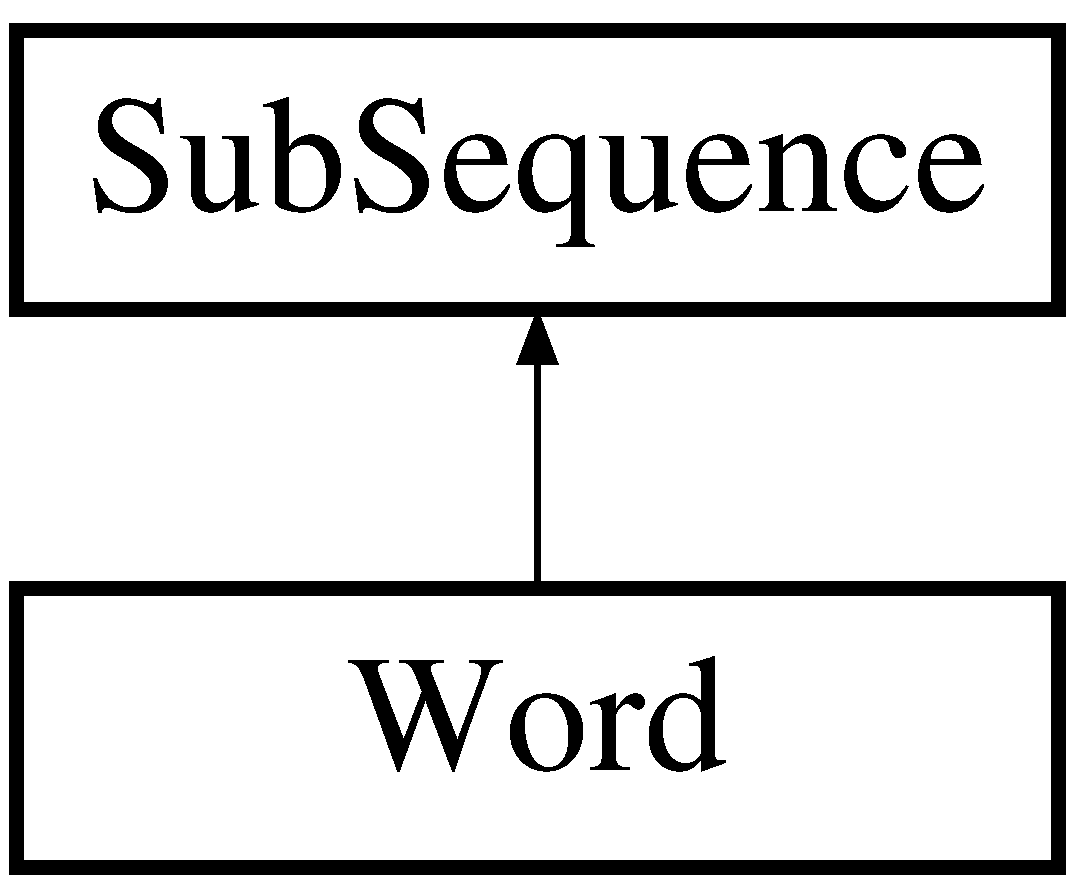
\includegraphics[height=2.000000cm]{classWord}
\end{center}
\end{figure}
\subsection*{Public Member Functions}
\begin{DoxyCompactItemize}
\item 
\hyperlink{classWord_ac4331ca9942a6730a472d6fa7c6d8924}{Word} (const shared\-\_\-ptr$<$ \hyperlink{classSequence}{Sequence} $>$ mother\-Seq, const int start, const int end, list$<$ int $>$ $\ast$occ\-Pos)
\item 
\hyperlink{classWord_a1fbcaae6859604d92e94cab540cb3523}{$\sim$\-Word} ()
\item 
list$<$ int $>$ $\ast$ \hyperlink{classWord_ac11d4329ae31c430d38fa37753f21e18}{get\-Occ\-Pos} () const 
\end{DoxyCompactItemize}
\subsection*{Friends}
\begin{DoxyCompactItemize}
\item 
ostream \& \hyperlink{classWord_a0dae9ce1ccead10392c7f5709b047b99}{operator$<$$<$} (ostream \&cout, const \hyperlink{classWord}{Word} \&w)
\end{DoxyCompactItemize}


\subsection{Constructor \& Destructor Documentation}
\hypertarget{classWord_ac4331ca9942a6730a472d6fa7c6d8924}{\index{Word@{Word}!Word@{Word}}
\index{Word@{Word}!Word@{Word}}
\subsubsection[{Word}]{\setlength{\rightskip}{0pt plus 5cm}Word\-::\-Word (
\begin{DoxyParamCaption}
\item[{const shared\-\_\-ptr$<$ {\bf Sequence} $>$}]{mother\-Seq, }
\item[{const int}]{start, }
\item[{const int}]{end, }
\item[{list$<$ int $>$ $\ast$}]{occ\-Pos}
\end{DoxyParamCaption}
)}}\label{classWord_ac4331ca9942a6730a472d6fa7c6d8924}
Itinialize father \hyperlink{classSubSequence}{Sub\-Sequence} class and assign occ\-Pos\-\_\- \hypertarget{classWord_a1fbcaae6859604d92e94cab540cb3523}{\index{Word@{Word}!$\sim$\-Word@{$\sim$\-Word}}
\index{$\sim$\-Word@{$\sim$\-Word}!Word@{Word}}
\subsubsection[{$\sim$\-Word}]{\setlength{\rightskip}{0pt plus 5cm}Word\-::$\sim$\-Word (
\begin{DoxyParamCaption}
{}
\end{DoxyParamCaption}
)}}\label{classWord_a1fbcaae6859604d92e94cab540cb3523}
Delete occ\-Pos\-\_\- list 

\subsection{Member Function Documentation}
\hypertarget{classWord_ac11d4329ae31c430d38fa37753f21e18}{\index{Word@{Word}!get\-Occ\-Pos@{get\-Occ\-Pos}}
\index{get\-Occ\-Pos@{get\-Occ\-Pos}!Word@{Word}}
\subsubsection[{get\-Occ\-Pos}]{\setlength{\rightskip}{0pt plus 5cm}list$<$ int $>$ $\ast$ Word\-::get\-Occ\-Pos (
\begin{DoxyParamCaption}
{}
\end{DoxyParamCaption}
) const}}\label{classWord_ac11d4329ae31c430d38fa37753f21e18}
get the word occs positions in \hyperlink{classSequence}{Sequence} \begin{DoxyReturn}{Returns}
occ\-Pos\-\_\- 
\end{DoxyReturn}


\subsection{Friends And Related Function Documentation}
\hypertarget{classWord_a0dae9ce1ccead10392c7f5709b047b99}{\index{Word@{Word}!operator$<$$<$@{operator$<$$<$}}
\index{operator$<$$<$@{operator$<$$<$}!Word@{Word}}
\subsubsection[{operator$<$$<$}]{\setlength{\rightskip}{0pt plus 5cm}ostream\& operator$<$$<$ (
\begin{DoxyParamCaption}
\item[{ostream \&}]{cout, }
\item[{const {\bf Word} \&}]{w}
\end{DoxyParamCaption}
)\hspace{0.3cm}{\ttfamily [friend]}}}\label{classWord_a0dae9ce1ccead10392c7f5709b047b99}
Overload $<$$<$ operator to cout the \hyperlink{classSubSequence}{Sub\-Sequence} 

The documentation for this class was generated from the following files\-:\begin{DoxyCompactItemize}
\item 
Word.\-h\item 
Word.\-cpp\end{DoxyCompactItemize}

\hypertarget{classWordList}{\section{Word\-List Class Reference}
\label{classWordList}\index{Word\-List@{Word\-List}}
}
\subsection*{Public Member Functions}
\begin{DoxyCompactItemize}
\item 
\hypertarget{classWordList_ad08a442d735959fa34bdcbdf83a03039}{{\bfseries Word\-List} (list$<$ shared\-\_\-ptr$<$ \hyperlink{classWord}{Word} $>$$>$ $\ast$word\-List)}\label{classWordList_ad08a442d735959fa34bdcbdf83a03039}

\item 
\hyperlink{classWordList_a51ee5b595a3812e94ea691120eb3df4e}{$\sim$\-Word\-List} ()
\item 
void \hyperlink{classWordList_a73e587d2f0c94919303c3873cecae43b}{insert} (shared\-\_\-ptr$<$ \hyperlink{classWord}{Word} $>$ w)
\item 
void \hyperlink{classWordList_a1526b6133bf3f55a802e431fe2e60c70}{set\-Occs\-Vec} (vector$<$ pair$<$ shared\-\_\-ptr$<$ \hyperlink{classWord}{Word} $>$, int $>$ $>$ v)
\item 
shared\-\_\-ptr$<$ \hyperlink{classWord}{Word} $>$ \hyperlink{classWordList_a9f2ec2dfb5f8670f9fc5420d2c9d3cfb}{find} (const shared\-\_\-ptr$<$ \hyperlink{classWord}{Word} $>$w) const 
\item 
list$<$ std\-::pair$<$ shared\-\_\-ptr\\*
$<$ \hyperlink{classWord}{Word} $>$, shared\-\_\-ptr$<$ \hyperlink{classWord}{Word} $>$ $>$ $>$ \hyperlink{classWordList_aee1a575e29d33758d632a601316fb803}{cross\-All\-Words} ()
\item 
int \hyperlink{classWordList_acba58ad886cc0029592df6c942b4dd2b}{sum\-Words\-Length\-With\-Repeats} () const 
\item 
int \hyperlink{classWordList_aedf495a6048450a25ac3754a0081f834}{sum\-Words\-Length\-Without\-Repeats} () const 
\item 
void \hyperlink{classWordList_aaab2e68dcf66a71ad5441c93266a1746}{clear} ()
\item 
list$<$ shared\-\_\-ptr$<$ \hyperlink{classWord}{Word} $>$ $>$ $\ast$ \hyperlink{classWordList_a2762e9ee93989472cf787b0cbda73cea}{get\-Word\-List} () const 
\item 
set$<$ shared\-\_\-ptr$<$ \hyperlink{classWord}{Word} $>$ $>$ $\ast$ \hyperlink{classWordList_afb3441c905e2b67dbc9b4e565e530c66}{get\-Word\-Set} () const 
\item 
\hypertarget{classWordList_a13390f6a405e412b79cab3586f5a7a48}{vector$<$ pair$<$ shared\-\_\-ptr$<$ \hyperlink{classWord}{Word} $>$\\*
, int $>$ $>$ {\bfseries get\-Word\-Vec} () const }\label{classWordList_a13390f6a405e412b79cab3586f5a7a48}

\item 
int \hyperlink{classWordList_a867573338edd050d6c121b4debe5276c}{word\-Pos} (shared\-\_\-ptr$<$ \hyperlink{classWord}{Word} $>$ w) const 
\item 
int \hyperlink{classWordList_a69eded9ac3a5f004f18413b68c3b5fd4}{get\-Size} () const 
\end{DoxyCompactItemize}
\subsection*{Friends}
\begin{DoxyCompactItemize}
\item 
ostream \& \hyperlink{classWordList_a70775d63dafa9f9c753f622bb6d945bf}{operator$<$$<$} (ostream \&cout, const \hyperlink{classWordList}{Word\-List} \&w\-S)
\end{DoxyCompactItemize}


\subsection{Constructor \& Destructor Documentation}
\hypertarget{classWordList_a51ee5b595a3812e94ea691120eb3df4e}{\index{Word\-List@{Word\-List}!$\sim$\-Word\-List@{$\sim$\-Word\-List}}
\index{$\sim$\-Word\-List@{$\sim$\-Word\-List}!WordList@{Word\-List}}
\subsubsection[{$\sim$\-Word\-List}]{\setlength{\rightskip}{0pt plus 5cm}Word\-List\-::$\sim$\-Word\-List (
\begin{DoxyParamCaption}
{}
\end{DoxyParamCaption}
)}}\label{classWordList_a51ee5b595a3812e94ea691120eb3df4e}
Delete word\-List\-\_\- list 

\subsection{Member Function Documentation}
\hypertarget{classWordList_aaab2e68dcf66a71ad5441c93266a1746}{\index{Word\-List@{Word\-List}!clear@{clear}}
\index{clear@{clear}!WordList@{Word\-List}}
\subsubsection[{clear}]{\setlength{\rightskip}{0pt plus 5cm}void Word\-List\-::clear (
\begin{DoxyParamCaption}
{}
\end{DoxyParamCaption}
)}}\label{classWordList_aaab2e68dcf66a71ad5441c93266a1746}
clear the Wordlist \hypertarget{classWordList_aee1a575e29d33758d632a601316fb803}{\index{Word\-List@{Word\-List}!cross\-All\-Words@{cross\-All\-Words}}
\index{cross\-All\-Words@{cross\-All\-Words}!WordList@{Word\-List}}
\subsubsection[{cross\-All\-Words}]{\setlength{\rightskip}{0pt plus 5cm}list$<$ std\-::pair$<$ shared\-\_\-ptr$<$ {\bf Word} $>$, shared\-\_\-ptr$<$ {\bf Word} $>$ $>$ $>$ Word\-List\-::cross\-All\-Words (
\begin{DoxyParamCaption}
{}
\end{DoxyParamCaption}
)}}\label{classWordList_aee1a575e29d33758d632a601316fb803}
Cross all elements of \hyperlink{classWordList}{Word\-List} \begin{DoxyReturn}{Returns}
list of words pairs representing cartesian product of elements 
\end{DoxyReturn}
\hypertarget{classWordList_a9f2ec2dfb5f8670f9fc5420d2c9d3cfb}{\index{Word\-List@{Word\-List}!find@{find}}
\index{find@{find}!WordList@{Word\-List}}
\subsubsection[{find}]{\setlength{\rightskip}{0pt plus 5cm}shared\-\_\-ptr$<$ {\bf Word} $>$ Word\-List\-::find (
\begin{DoxyParamCaption}
\item[{const shared\-\_\-ptr$<$ {\bf Word} $>$}]{w}
\end{DoxyParamCaption}
) const}}\label{classWordList_a9f2ec2dfb5f8670f9fc5420d2c9d3cfb}
find if there is another ptr pointing to same object, if exists return it 
\begin{DoxyParams}{Parameters}
{\em w} & ptr to searching w \\
\hline
\end{DoxyParams}
\begin{DoxyReturn}{Returns}
ptr to existing one or N\-U\-L\-L if it doesnt exist. 
\end{DoxyReturn}
\hypertarget{classWordList_a69eded9ac3a5f004f18413b68c3b5fd4}{\index{Word\-List@{Word\-List}!get\-Size@{get\-Size}}
\index{get\-Size@{get\-Size}!WordList@{Word\-List}}
\subsubsection[{get\-Size}]{\setlength{\rightskip}{0pt plus 5cm}int Word\-List\-::get\-Size (
\begin{DoxyParamCaption}
{}
\end{DoxyParamCaption}
) const}}\label{classWordList_a69eded9ac3a5f004f18413b68c3b5fd4}
get the word\-List size \begin{DoxyReturn}{Returns}
size\-\_\- 
\end{DoxyReturn}
\hypertarget{classWordList_a2762e9ee93989472cf787b0cbda73cea}{\index{Word\-List@{Word\-List}!get\-Word\-List@{get\-Word\-List}}
\index{get\-Word\-List@{get\-Word\-List}!WordList@{Word\-List}}
\subsubsection[{get\-Word\-List}]{\setlength{\rightskip}{0pt plus 5cm}list$<$ shared\-\_\-ptr$<$ {\bf Word} $>$ $>$ $\ast$ Word\-List\-::get\-Word\-List (
\begin{DoxyParamCaption}
{}
\end{DoxyParamCaption}
) const}}\label{classWordList_a2762e9ee93989472cf787b0cbda73cea}
get the word\-List \begin{DoxyReturn}{Returns}
word\-List\-\_\- 
\end{DoxyReturn}
\hypertarget{classWordList_afb3441c905e2b67dbc9b4e565e530c66}{\index{Word\-List@{Word\-List}!get\-Word\-Set@{get\-Word\-Set}}
\index{get\-Word\-Set@{get\-Word\-Set}!WordList@{Word\-List}}
\subsubsection[{get\-Word\-Set}]{\setlength{\rightskip}{0pt plus 5cm}set$<$ shared\-\_\-ptr$<$ {\bf Word} $>$ $>$ $\ast$ Word\-List\-::get\-Word\-Set (
\begin{DoxyParamCaption}
{}
\end{DoxyParamCaption}
) const}}\label{classWordList_afb3441c905e2b67dbc9b4e565e530c66}
get the word\-Set \begin{DoxyReturn}{Returns}
word\-Set\-\_\- 
\end{DoxyReturn}
\hypertarget{classWordList_a73e587d2f0c94919303c3873cecae43b}{\index{Word\-List@{Word\-List}!insert@{insert}}
\index{insert@{insert}!WordList@{Word\-List}}
\subsubsection[{insert}]{\setlength{\rightskip}{0pt plus 5cm}void Word\-List\-::insert (
\begin{DoxyParamCaption}
\item[{shared\-\_\-ptr$<$ {\bf Word} $>$}]{w}
\end{DoxyParamCaption}
)}}\label{classWordList_a73e587d2f0c94919303c3873cecae43b}
Insert a word in the word\-List 
\begin{DoxyParams}{Parameters}
{\em w} & word to be inserted \\
\hline
\end{DoxyParams}
\hypertarget{classWordList_a1526b6133bf3f55a802e431fe2e60c70}{\index{Word\-List@{Word\-List}!set\-Occs\-Vec@{set\-Occs\-Vec}}
\index{set\-Occs\-Vec@{set\-Occs\-Vec}!WordList@{Word\-List}}
\subsubsection[{set\-Occs\-Vec}]{\setlength{\rightskip}{0pt plus 5cm}void Word\-List\-::set\-Occs\-Vec (
\begin{DoxyParamCaption}
\item[{vector$<$ pair$<$ shared\-\_\-ptr$<$ {\bf Word} $>$, int $>$ $>$}]{v}
\end{DoxyParamCaption}
)}}\label{classWordList_a1526b6133bf3f55a802e431fe2e60c70}
Set the occurences vector of the \hyperlink{classWordList}{Word\-List} 
\begin{DoxyParams}{Parameters}
{\em v} & vector of ocurrences \\
\hline
\end{DoxyParams}
\hypertarget{classWordList_aedf495a6048450a25ac3754a0081f834}{\index{Word\-List@{Word\-List}!sum\-Words\-Length\-Without\-Repeats@{sum\-Words\-Length\-Without\-Repeats}}
\index{sum\-Words\-Length\-Without\-Repeats@{sum\-Words\-Length\-Without\-Repeats}!WordList@{Word\-List}}
\subsubsection[{sum\-Words\-Length\-Without\-Repeats}]{\setlength{\rightskip}{0pt plus 5cm}int Word\-List\-::sum\-Words\-Length\-Without\-Repeats (
\begin{DoxyParamCaption}
{}
\end{DoxyParamCaption}
) const}}\label{classWordList_aedf495a6048450a25ac3754a0081f834}
Sum all the words length without repeating words \begin{DoxyReturn}{Returns}
sum 
\end{DoxyReturn}
\hypertarget{classWordList_acba58ad886cc0029592df6c942b4dd2b}{\index{Word\-List@{Word\-List}!sum\-Words\-Length\-With\-Repeats@{sum\-Words\-Length\-With\-Repeats}}
\index{sum\-Words\-Length\-With\-Repeats@{sum\-Words\-Length\-With\-Repeats}!WordList@{Word\-List}}
\subsubsection[{sum\-Words\-Length\-With\-Repeats}]{\setlength{\rightskip}{0pt plus 5cm}int Word\-List\-::sum\-Words\-Length\-With\-Repeats (
\begin{DoxyParamCaption}
{}
\end{DoxyParamCaption}
) const}}\label{classWordList_acba58ad886cc0029592df6c942b4dd2b}
Sum all the words lenght of the wordlist \begin{DoxyReturn}{Returns}
sum 
\end{DoxyReturn}
\hypertarget{classWordList_a867573338edd050d6c121b4debe5276c}{\index{Word\-List@{Word\-List}!word\-Pos@{word\-Pos}}
\index{word\-Pos@{word\-Pos}!WordList@{Word\-List}}
\subsubsection[{word\-Pos}]{\setlength{\rightskip}{0pt plus 5cm}int Word\-List\-::word\-Pos (
\begin{DoxyParamCaption}
\item[{shared\-\_\-ptr$<$ {\bf Word} $>$}]{w}
\end{DoxyParamCaption}
) const}}\label{classWordList_a867573338edd050d6c121b4debe5276c}
get the word position in the \hyperlink{classWordList}{Word\-List} 
\begin{DoxyParams}{Parameters}
{\em w} & word \\
\hline
\end{DoxyParams}
\begin{DoxyReturn}{Returns}
pos 
\end{DoxyReturn}


\subsection{Friends And Related Function Documentation}
\hypertarget{classWordList_a70775d63dafa9f9c753f622bb6d945bf}{\index{Word\-List@{Word\-List}!operator$<$$<$@{operator$<$$<$}}
\index{operator$<$$<$@{operator$<$$<$}!WordList@{Word\-List}}
\subsubsection[{operator$<$$<$}]{\setlength{\rightskip}{0pt plus 5cm}ostream\& operator$<$$<$ (
\begin{DoxyParamCaption}
\item[{ostream \&}]{cout, }
\item[{const {\bf Word\-List} \&}]{w\-S}
\end{DoxyParamCaption}
)\hspace{0.3cm}{\ttfamily [friend]}}}\label{classWordList_a70775d63dafa9f9c753f622bb6d945bf}
Overload $<$$<$ operator to cout the \hyperlink{classWordList}{Word\-List} 

The documentation for this class was generated from the following files\-:\begin{DoxyCompactItemize}
\item 
Word\-List.\-h\item 
Word\-List.\-cpp\end{DoxyCompactItemize}

%--- End generated contents ---

% Index
\newpage
\phantomsection
\addcontentsline{toc}{chapter}{Index}
\printindex

\end{document}
